%%%%%%%%%%%%%%%%%%%%%%%%%%%%%%%%%%%%%%%%%
% Masters/Doctoral Thesis 
% LaTeX Template
% Version 2.5 (27/8/17)
%
% This template was downloaded from:
% http://www.LaTeXTemplates.com
%
% Version 2.x major modifications by:
% Vel (vel@latextemplates.com)
%
% This template is based on a template by:
% Steve Gunn (http://users.ecs.soton.ac.uk/srg/softwaretools/document/templates/)
% Sunil Patel (http://www.sunilpatel.co.uk/thesis-template/)
%
% Template license:
% CC BY-NC-SA 3.0 (http://creativecommons.org/licenses/by-nc-sa/3.0/)
%
%%%%%%%%%%%%%%%%%%%%%%%%%%%%%%%%%%%%%%%%%

%----------------------------------------------------------------------------------------
%	PACKAGES AND OTHER DOCUMENT CONFIGURATIONS
%----------------------------------------------------------------------------------------
\documentclass[
11pt, % The default document font size, options: 10pt, 11pt, 12pt
%oneside, % Two side (alternating margins) for binding by default, uncomment to switch to one side
ngerman, % ngerman for German
singlespacing, % Single line spacing, alternatives: onehalfspacing or doublespacing
%draft, % Uncomment to enable draft mode (no pictures, no links, overfull hboxes indicated)
%nolistspacing, % If the document is onehalfspacing or doublespacing, uncomment this to set spacing in lists to single
%liststotoc, % Uncomment to add the list of figures/tables/etc to the table of contents
%toctotoc, % Uncomment to add the main table of contents to the table of contents
%parskip, % Uncomment to add space between paragraphs
%nohyperref, % Uncomment to not load the hyperref package
headsepline, % Uncomment to get a line under the header
%chapterinoneline, % Uncomment to place the chapter title next to the number on one line
%consistentlayout, % Uncomment to change the layout of the declaration, abstract and acknowledgements pages to match the default layout
]{MastersDoctoralThesis} % The class file specifying the document structure
\usepackage{float}
\usepackage{caption}
\usepackage{fancyvrb}
\usepackage{enumitem}
\usepackage{capt-of}

\usepackage{pgfplots}
\pgfplotsset{width=7cm,compat=1.8}
\usepackage[utf8]{inputenc} % Required for inputting international characters
\usepackage[T1]{fontenc} % Output font encoding for international characters
\usepackage[colorlinks]{hyperref}
\usepackage{mathpazo} % Use the Palatino font by default

\usepackage{graphicx}
\usepackage{placeins}
\usepackage[backend=bibtex,style=authoryear,natbib=true]{biblatex} % Use the bibtex backend with the authoryear citation style (which resembles APA)

\addbibresource{example.bib} % The filename of the bibliography

\usepackage[autostyle=true]{csquotes} % Required to generate language-dependent quotes in the bibliography

%----------------------------------------------------------------------------------------
%	MARGIN SETTINGS
%----------------------------------------------------------------------------------------

\geometry{
	paper=a4paper, % Change to letterpaper for US letter
	inner=2.5cm, % Inner margin
	outer=3.8cm, % Outer margin
	bindingoffset=.5cm, % Binding offset
	top=1.5cm, % Top margin
	bottom=3cm, % Bottom margin
	%showframe, % Uncomment to show how the type block is set on the page
}

%----------------------------------------------------------------------------------------
%	THESIS INFORMATION
%----------------------------------------------------------------------------------------

\thesistitle{Evaluierung von temporalen Graphdatenbanken am Beispiel von Neo4j} % Your thesis title, this is used in the title and abstract, print it elsewhere with \ttitle
\supervisor{Prof. Dr. Ralf Möller \textsc{Smith}} % Your supervisor's name, this is used in the title page, print it elsewhere with \supname
\examiner{} % Your examiner's name, this is not currently used anywhere in the template, print it elsewhere with \examname
\degree{Bachelor of Science} % Your degree name, this is used in the title page and abstract, print it elsewhere with \degreename
\author{Ove Folger} % Your name, this is used in the title page and abstract, print it elsewhere with \authorname
\addresses{} % Your address, this is not currently used anywhere in the template, print it elsewhere with \addressname

\subject{Graphdatabases} % Your subject area, this is not currently used anywhere in the template, print it elsewhere with \subjectname
\keywords{} % Keywords for your thesis, this is not currently used anywhere in the template, print it elsewhere with \keywordnames
\university{\href{https://www.uni-luebeck.de/universitaet/universitaet.html}{Universität zu Lübeck}} % Your university's name and URL, this is used in the title page and abstract, print it elsewhere with \univname
\department{\href{https://www.ifis.uni-luebeck.de/}{Institut für Informationssysteme}} % Your department's name and URL, this is used in the title page and abstract, print it elsewhere with \deptname
\group{\href{https://www.ifis.uni-luebeck.de/}{Institut für Informationssysteme}} % Your research group's name and URL, this is used in the title page, print it elsewhere with \groupname
\faculty{\href{https://www.uni-luebeck.de/structure/sektionen/informatiktechnik.html}{Sektion Informatik/Technik}} % Your faculty's name and URL, this is used in the title page and abstract, print it elsewhere with \facname

\AtBeginDocument{
\hypersetup{pdftitle=\ttitle} % Set the PDF's title to your title
\hypersetup{pdfauthor=\authorname} % Set the PDF's author to your name
\hypersetup{pdfkeywords=\keywordnames} % Set the PDF's keywords to your keywords
}

\begin{document}
\frontmatter % Use roman page numbering style (i, ii, iii, iv...) for the pre-content pages

\pagestyle{plain} % Default to the plain heading style until the thesis style is called for the body content

%----------------------------------------------------------------------------------------
%	TITLE PAGE
%----------------------------------------------------------------------------------------

\begin{titlepage}

	\Large
	\title{Evaluierung von temporalen Graphdatenbanken am Beispiel von Neo4j }
	
\includegraphics[width=8cm]{Figures/ifis_logo.png}
	\vskip 44pt
		 \noindent {\LARGE Evaluierung von temporalen Graphdatenbanken am Beispiel von Neo4j \par}
		\vskip 20pt
	\noindent	\textbf{Bachelorarbeit}
		\vskip 20pt
	 \noindent	im Rahmen des Studiengangs \\
		\textbf{Medieninformatik} \\
		der Universität zu Lübeck
		\vskip 20pt
		\noindent vorgelegt von \\
		\textbf{Ove Folger}
		\vskip 20pt
	\noindent	ausgegeben und betreut von \\
		\textbf{Prof. Dr. Ralf Möller}
		\vfill
		Lübeck, den \today
		\vskip 20pt


\end{titlepage}

%----------------------------------------------------------------------------------------
%	DECLARATION PAGE
%----------------------------------------------------------------------------------------
\begin{declaration}

	\bigskip\noindent Hiermit erkl{\"a}re ich an Eides statt, dass
	ich die vorliegende Arbeit selbst\-st{\"a}n\-dig verfasst und keine
	anderen als die angegebenen Quellen und Hilfsmittel verwendet habe.\par
	\bigskip\noindent Luebeck, \today
	\vskip 10mm
	\hfill\rule{18em}{.3pt}%
\end{declaration}





%----------------------------------------------------------------------------------------
%	ABSTRACT PAGE
%----------------------------------------------------------------------------------------

\begin{abstract}
	Durch das steigende Interesse an der Analyse von vernetzten Informationen werden Datenbanken des NoSQL-Ansatzes weiterentwickelt und für diese Analyse genutzt \parencite{angles2018property}. Eine Untergruppe dieses Ansatzes stellen die Graphdatenbanken dar, einer der populärsten Vertreter dieser Gruppe ist Neo4j. In dieser Arbeit wird beschrieben, wie sich die Performanz des System Neo4j bei der Bearbeitung von verschiedenen Anfragen verhält. Zu diesem Zweck wurden mehrere Anfragen mit semantisch gleichen Vergleichsanfragen an Neo4j gestellt und die Differenz der Bearbeitungszeiten wurde analysiert. Jede Anfrage wurde einer oder mehreren Kategorien zugeordnet, um so eine Korrelation zwischen Kategorie und Bearbeitungszeit einer Anfrage zu erkennen. \newline
	Für eine Einordnung der Performanz von Neo4j wurden alle aufgestellten Anfragen ebenfalls auf dem Datenbankmanagementsystem OrientDB ausgeführt\parencite{OrientDB}. Die Analyse zeigt, dass Neo4j die vorgestellten Anfragen mit der eigenen Anfragesprache Cypher durchschnittlich ca.1,9 mal schneller bearbeitete als OrientDB mit SQL. Neo4j kann für eine erhöhte Performanz in Java bedient werden, die Anfragen wurden in Java ca. 207 mal schneller als in OrientDB bearbeitet. Es konnte keine allgemeine Korrelation zwischen Kategorie einer Anfrage und ihrer Bearbeitungszeit in Neo4j festgestellt werden. Für das Speichern des Datensatzes benötigte Neo4j ca. 2,4 mal mehr Speicherplatz als OrientDB. Die Nutzungsvielfalt und gute Performanz wurden als Stärke und die schlechte Speicherverwaltung als Schwäche von Neo4j hervorgehoben. \newline
	\begin{center}
		\textbf{Evaluation of temporal graph databases using the example of Neo4j}
	\end{center}
	Due to the increasing interest in analyzing networked information, databases of the NoSQL approach are further developed and used for this analysis \parencite{angles2018property}. A subset of this approach is represented by the graph databases, one of the most popular members of this group is Neo4j. This work describes how the performance of the Neo4j system behaves when handling various requests. For this purpose, several queries with semantically equal comparison queries were processed on the system and the difference of processing times was analyzed. Each query has been assigned to one or more categories to detect a correlation between the category and the processing time of a query. \newline
	In order to rank the performance of Neo4j, all queries  were also executed on the databasemanagementsystem OrientDB \parencite{OrientDB}. The analysis shows that Neo4j processed the requested queries with its own query language Cypher on average about 1.9 times faster than OrientDB with SQL. Neo4j can be used for increased performance in Java, the queries were processed in Java about 207 times faster than in OrientDB. There was no general correlation between the category of a query and its processing time in Neo4j. Neo4j needed about 2.4 times more memory than the OrientDB to save the dataset. The versatility and good performance were highlighted as a strength and the poor memory management as a weakness of Neo4j.	
\end{abstract}




%----------------------------------------------------------------------------------------
%	LIST OF CONTENTS/FIGURES/TABLES PAGES
%----------------------------------------------------------------------------------------

{
	\setcounter{tocdepth}{1}
	\hypersetup{linkcolor=black}
	\tableofcontents
}

\hypersetup{linkcolor= black}
\listoffigures % Prints the list of figures


\listoftables % Prints the list of tables
%----------------------------------------------------------------------------------------
%	ABBREVIATIONS
%----------------------------------------------------------------------------------------

\begin{abbreviations}{ll} % Include a list of abbreviations (a table of two columns)
	
	\textbf{SQL} & \textbf{S}tructured \textbf{Q}uery \textbf{L}anguage\\
	\textbf{NoSQL} & \textbf{N}ot \textbf{o}nly \textbf{SQL}\\
	\textbf{GDB} & \textbf{G}raph \textbf{D}ata\textbf{b}ase \\
	\textbf{API} & \textbf{A}pplication \textbf{P}rogramming \textbf{I}nterface \\
	\textbf{DBMS} & \textbf{D}ata\textbf{b}ase\textbf{m}anagement\textbf{s}ystem \\
	\textbf{UDF} & \textbf{U}ser \textbf{D}efined \textbf{F}unctions \\
	\textbf{APOC} & \textbf{A}wesome \textbf{P}rocedures \textbf{o}n \textbf{C}ypher\\
	\textbf{ACID} & \textbf{A}tomicity \textbf{C}onsistency \textbf{I}solation \textbf{D}urability\\
	\textbf{CAP} & \textbf{C}onsistency \textbf{A}vailibility \textbf{P}artition Tolerance  \\
	\textbf{LFU} &\textbf{L}east \textbf{F}requently \textbf{U}sed \\
	\textbf{ASB} & \textbf{A}bstrakter \textbf{S}yntax \textbf{B}aum\\
	\textbf{GUI} & \textbf{G}rafisches \textbf{U}ser \textbf{I}nterface\\
	\textbf{HTTP} & \textbf{H}yper\textbf{t}ext \textbf{T}ransfer \textbf{P}rotocol\\
	\textbf{LFU} & \textbf{l}east\textbf{f}requently \textbf{u}sed\\
	\textbf{JVM} & \textbf{J}ava\textbf{v}irtual \textbf{m}achine\\

\end{abbreviations}
%----------------------------------------------------------------------------------------
%	DEDICATION
%----------------------------------------------------------------------------------------

%----------------------------------------------------------------------------------------
%	THESIS CONTENT - CHAPTERS
%----------------------------------------------------------------------------------------

\mainmatter % Begin numeric (1,2,3...) page numbering

\pagestyle{thesis} % Return the page headers back to the "thesis" style
% Include the chapters of the thesis as separate files from the Chapters folder
% Uncomment the lines as you write the chapters
% Chapter 0

\chapter{Hintergrund} % Main chapter title

\label{Kaptiel1} % For referencing the chapter elsewhere, use \ref{Chapter1} 

%----------------------------------------------------------------------------------------

% Define some commands to keep the formatting separated from the content 
\newcommand{\keyword}[1]{\textit{#1}}
\newcommand{\tabhead}[1]{\textbf{#1}}
\newcommand{\code}[1]{\texttt{#1}}
\newcommand{\file}[1]{\texttt{\bfseries#1}}
\newcommand{\option}[1]{\texttt{\itshape#1}}

Um Daten in einer Datenbank abzulegen ist ein Datenmodell nötig, welches  das Allgemeine Verhalten der Datenbank definiert. Dieses ist durch folgende Eigenschaften definiert ist: ein Liste von Datenstruktur Typen, ein Liste von Operatoren die auf die Daten angewandt werden können und eine Liste der Regeln zur Vollständigkeit der Datenbank \parencite{codd1981data}. Zwei dieser Datenmodelle sind der Relationale-Ansatz und die NoSQL-Bewegung. Die meisten Datenbanken werden heutzutage nach dem relationalen Datenmodell verwaltet und mittels SQL bearbeitet \parencite{miller2013graph}. Dieses Schema wurde über viele Jahre lang optimiert und gilt für viele Daten als performanteste Implementierung \parencite{miller2013graph}. Die verwendete Datenstruktur bildet eine Tabelle, eine Reihe bildet ein Objekt und die Spalten bilden die dazugehörigen Attribute \parencite{miller2013graph}. Die Möglichkeiten der Operationen, mit denen die Daten verändert oder angefragt werden,sind durch den SQL-Standard bzw. die Implementierung des  Standards limitiert. Die Regeln zur Vollständigkeit der Datenbank sind ebenfalls im Standard festgehalten.  Als eine Alternative zu diesem relationalen Datenmodell gibt es die “NoSQL” Bewegung, welche erstmal 1998 erwähnt wurde \parencite{strauch2011nosql}. Diese Bewegung versuchte zunächst den Gebrauch von SQL als Anfragesprache zu vermeiden und brachte in den folgenden Jahren weitere Datenmodelle hervor. Eines dieser Konzepte ist das Darstellen von Daten in der Datenstruktur eines Graphen \parencite{miller2013graph}. Die sogenannten Graphdatenbanken(GDB) werden besonders in dem Darstellen von Netzwerken verwendet \parencite{han2011survey}, da das relationalen Datenmodell bei großen Datenmengen und vielen komplex verbunden Informationen durch eine hohe Anzahl von notwendigen Joins nicht performant verwendet werden kann \parencite{miller2013graph}. Für GDBs gibt es keine standardisierte Anfragesprache und  die Menge an möglichen Operatoren ist sehr variable. Neo4j ist ein populäres Beispiel für Graphdatenbanken und wird im folgenden genauer beschrieben.


% Chapter Template

\chapter{Grundlagen} % Main chapter title

\label{Kaptiel3} % Change X to a consecutive number; for referencing this chapter elsewhere, use \ref{ChapterX}

%----------------------------------------------------------------------------------------
%	SECTION 1
%----------------------------------------------------------------------------------------
\section{Graph}

Ein Graph ist eine abstrakte Datenstruktur, welche für die GDBs verwendet werden \parencite{vicknair2010comparison}. Ein Graph besteht aus einer endlichen nicht leeren Summe von Knoten, auch Vertex oder Punkte genannt und Kanten. Die Kanten des Graphen bildet die Verbindung zwischen zwei Knoten \url{ http://wwwmayr.in.tum.de/lehre/2008WS/ea/EA-7.pdf}(7.06.19), wenn die Kanten aus einem geordneten Paar bestehen und somit eine Richtung besitzen wird der Graph als gerichtet bezeichnet, bei einem ungeordneten Paar wird von einem ungerichteten Graph gesprochen\parencite{bondy1976graph}. Wenn die Kanten Attribute, wie zum Beispiel Kosten besitzen wird der Graph als gewichtet bezeichnet und ohne Attribute als ungewichtet  \url{ http://wwwmayr.in.tum.de/lehre/2008WS/ea/EA-7.pdf}(7.06.19). 

%-----------------------------------
%	SUBSECTION 1
%-----------------------------------
\section{Neo4j}

Neo4j ist eine Graphdatenbank, welche in Java implementiert wurde \parencite{vukotic2015neo4j}. Als Grundlegende Datenstruktur wird ein gerichteter und gewichteter  Graph verwendet.Knoten stellen die Entitäten,beispielsweise eine Person oder ein Produkt,  da und  Kanten stellen die Relationen zwischen den Entitäten da, beispielsweise “isAngestellt” und können optional ein Gewicht und eine Richtung besitzen. Attribute können als zusätzliche Informationen in den Knoten gespeichert  werden wie zum Beispiel: Name bei einem Knoten “Person”. Knoten können mit Bezeichnern versehen werden, um so leichter in Anfragen  verwendet werden zu können. Die Operationen sind entweder durch durch die  Anfragesprache  Cypher,welche eine standardisierten Syntax mit  mehreren vordefinierten Funktionen besitzt, limitiert oder durch die jeweilige verwendete Programmiersprache.Es wird das Einbetten weiterer Bibliotheken, welche weitere Funktionen oder Algorithmen stellen, unterstützt. Durch weitere Funktionen wie zum Beispiel die Bibliothek “APOC” \footnote{https://neo4j-contrib.github.io/neo4j-apoc-procedures/ (17.05.19) } ist es möglich, Daten aus verschiedenen Formaten wie JSON,XSL oder XML in die Datenbank zu laden oder Daten aus anderen Web-APIs zu nutzen. Neo4j lässt sich in einem  eingebetteten Modus oder einem  Server Modus nutzen. Der eingebettete Modus dient der direkten  Nutzung durch die Java Core API(Application programming interface)  von Neo4j. Der Server Modus ermöglicht eine getrennte Ausführung von dem Code und dem bestehenden Neo4j System.

\section{Neo4j als Datenbank management system}
Ein Datenbank Managment System(DBMS), ist für die Verarbeitung von Anfragen verantwortlich und kann mit folgenden Teilen beschrieben werden: Eine Schnittstelle mit dem Nutzer, eine Anfragesprache, ein Anfrage-Optimierer, eine storage engine ,eine transaction engine, eine database engine und operation features, zum Wiederherstellen von Daten \parencite{angles2012comparison}. Als Schnittstelle mit dem Nutzer stehen die Anwendungen “Neo4j Browser” unter Linux und “Neo4j Desktop” unter Windows zur Verfügung, zusätzlich besteht die Möglichkeit eine von den Neo4j Treibern unterstützte Programmiersprache  oder Java zu verwenden und direkt die Neo4j APIs zu nutzen. Die Anfragesprache für Neo4j Browser und Neo4j Desktop ist “Cypher”. Zum Optimieren von Anfrageplänen wird der “Cypher Query Optimizer”verwendet. Die wird storage engine durch die Record Files und die transaction unit  wird durch das Transaction Management dargestellt. Die database engine bildet das Gesamtsystem der einzelnen Komponenten. Die operation features zum Wiederherstellen von Daten werden in dem Transaktions-Log realisiert. Optional kann zu eventuellen Performanz Steigerung ein Cache verwaltet werden. In der Neo4j Enterprise Version ist es möglich, das DBMS auf mehrere Systeme in einem Netzwerk mittels High Availability Funktion auszulagern \parencite{vukotic2015neo4j}. Zusammengefasst wird die Architektur in \ref{fig:Architecure}

\begin{figure}[th]
	\centering
	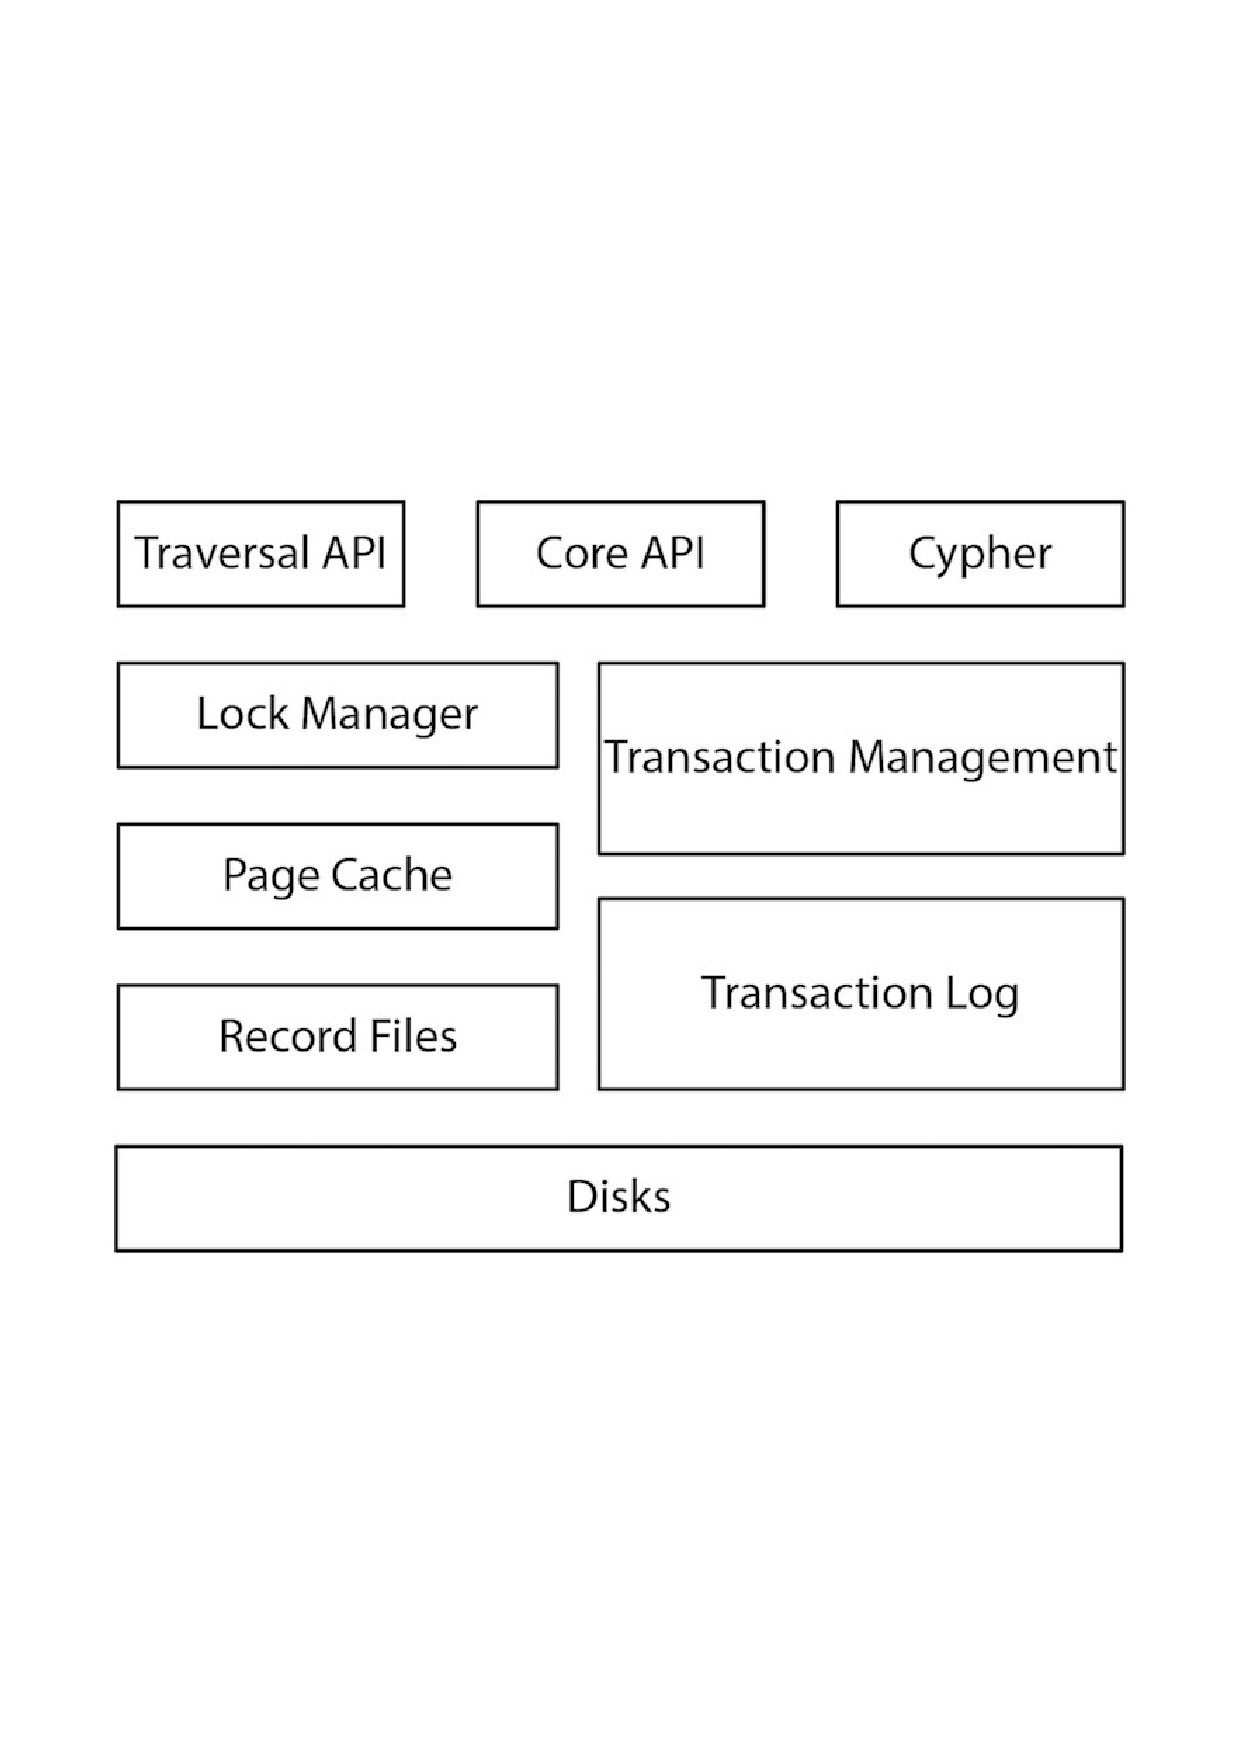
\includegraphics [width=13cm, height=14cm]{Figures/Architecure}
	\caption[Architecture]{Allgemeine Architektur von Neo4j.}
	\label{fig:Architecure}
\end{figure}

\subsection{Cypher und APIs für Neo4j}
Im Folgenden werden die Möglichkeiten zum Interagieren mit Neo4j beschrieben. Da es über die Neo4j-Treiber möglich ist, Neo4j in mehreren Programmiersprachen zu nutzen und die genaue Anzahl der Sprachen stetig steigt, werden im folgenden nur die Kernfunktionen in Java beschrieben und verwendet. Im späteren Absatz zu Neo4j im Servermodus wird zusätzlich das Bolt-protocol und die REST HTTP API beschrieben, welche als weitere Schnittstelle dienen.

\subsubsection{Cypher}
Im Gegensatz zu den relationalen Datenbanken gibt es bei Graphdatenbanken keine standardisierte Anfragesprache, welche bei den meisten Graphdatenbanken Verwendung findet \parencite{han2011survey}. In Neo4j besteht seit 2000 die Möglichkeit die deklarative Anfragesprache “Cypher” zu verwendenden  \parencite{francis2018cypher}. Cypher wird von Neo4, Inc. entwickelt und wurde ursprünglich ausschließlich für die Neo4j Datenbank verwendet. Seit Oktober 2015  findet Cypher als “openCypher” Gebrauch in anderen Datenbanken \parencite{francis2018cypher}. Da für die Traversal API und die Java Core API Kenntnisse in Java bzw. einer durch die Neo4j-Treiber unterstützten Programmiersprachen benötigt werden, bildet Cypher eine Möglichkeit ohne diese Kenntnisse mit der Datenbank zu interagieren[16]. Die Syntax ist an SQL und Gremlin \parencite{vukotic2015neo4j} orientiert. In Cypher wird ein Muster von dem Nutzer angegeben und alle Objekte, die dieses Muster erfüllen, können zurückgegeben werden. Die wichtigsten  Schlüsselwörter sind: \newline
\textbf{Where}: Dies hat die gleiche Funktion wie in SQL und spezifiziert Objekte durch einen Ausdruck. \newline
\textbf{Match}: Dadurch wird das Muster spezifiziert indem Neo4j suchen soll. Beispielweise: 
\begin{Verbatim}[frame=single]
MATCH (p1:Person)-[:Friends]->(p2:Person) 
WHERE p1.name= ‘Peter’ 
RETURN p.name
\end{Verbatim}
, hier werden alle Personen-Knoten durchsucht, die mit einer “Friends”-Relation mit dem Personen-Knoten von “Peter” verbunden sind. p1 stellt ein Label für den Knoten vom Typ “Person” da, [:Friends] ist eine Relation vom Typ “Friends” und durch “->” wird angegeben, dass es sich um eine ausgehende Kante vom Knoten p1 handelt. \newline
\textbf{Return}: Es wird angegeben, welche Objekte bzw. welche Attribute der Objekte, die das Muster erfüllen zurückgegeben werden sollen.\newline
\textbf{Delete}: Wie in SQL  wird ein Objekt  oder mehrere Objekte aus der Datenbank entfernt.\newline
\textbf{With}: Dadurch lassen sich in einer Anfrage Objekte manipulieren bevor sie zu einer weiteren Anfrage gegeben werden. Beispielsweise:
\begin{Verbatim}[frame=single]
MATCH (p:Person{name: ‘Peter’})  
WITH COUNT(p) as count  
RETURN count
\end{Verbatim} 
\textbf{Create}: Erzeugt ein Objekt in der Datenbank Beispielsweise 
\begin{Verbatim}[frame=single]
Create (p:Person)
\end{Verbatim}
, hier wird ein Knoten vom Typ Person erzeugt. Es ist auch möglich mehrere Knoten mit den dazugehörigen Relationen zu erzeugen. Indizes  für die Objekte oder Attribute von Objekten können ebenfalls über Create erzeugt werden.\newline
\textbf{Limit}: Beschränkt die Menge, welche durch das Return-Statement zurückgegeben wird Beispielsweise
\begin{Verbatim}[frame=single]
MATCH (p:person) RETURN p.name LIMIT 10
\end{Verbatim} 
, hier werden nur die Namen  von 10 Personen zurückgegeben\newline
\textbf{SUM/COUNT/AVG}: Werden wie in SQL verwendet. \newline
Der Nutzer beeinflusst so welche Daten durch  das Musters gesucht werden. Der Nutzer besitzt keine Möglichkeit die Art der Berechnung zu beeinflussen. Cypher wird dadurch als Nutzerfreundlichere, aber auch weniger performante Alternative zu den APIs empfohlen \parencite{vukotic2015neo4j}. In den folgenden Experimenten wurde sowohl Cypher als als auch die Travese API für einen direkten Vergleich verwendet. Cypher lässt sich ausschließlich als single thread ausführen.

\subsubsection{Java Core API}
Als low-level Schnittstelle zu den Kernfunktionen von Neo4j ist dies die Möglichkeit mit der besten Laufzeit \parencite{vukotic2015neo4j}. Zur Verwendung dieser imperativen API sind weitreichende Programmierkenntnisse und Wissen über die Neo4j-Bibliotheken, sowie einer genauen Vorstellung über die Daten in dem Graph erforderlich. Wenn diese Kenntnisse gegeben sind, ist die API sehr flexible verwendbar  und der Nutzer hat hohen Einfluss darauf, wie die Anfragen bearbeitet werden sollen und kann so eine optimale Berechnungsstrategie angeben \parencite{vukotic2015neo4j}. Die so produzierten Queries sind in meisten sehr lang. Eine Beispielhafte Berechung wäre:
\begin{Verbatim}[frame=single]
try ( Transaction tx = graphDb.beginTx() )
{
	Node Peter = graphDb.getNodeById(Peter_ID);
	Set<Node> friends = new HashSet<Node>();
	for (Relationship R : Peter.getRelationships(FRIEND)) {  
		Node friend = R.getOtherNode(userJohn);
		friends.add(friend);                        
	}
	for (Node friend : friends) {
	  logger.info("Found friend: " + friend.getProperty("name")); 
}

\end{Verbatim}
Bei diesem Beispiel werden alle Freunde von Peter gefunden und zurückgegeben.Der Nutzer gibt jede Transaktion explizit an,so ist es dem System möglich alle zur Verfügung stehenden Kerne zu nutzen.

\subsubsection{Traversal API}
Diese deklarative API  dient zum spezifizieren von Traversierungen im Graph, sie ist schneller als Cypher und langsamer als die Core API. Die Traversal API erlaubt einen high-level Zugriff auf Neo4j, welcher weniger abstrakt als die Core API ist und dennoch Programmierkenntnisse erfordert. Der Nutzer muss keine genaue Vorstellung von den Daten im Graphen haben.Es wird eine Beschreibung angegeben, wie eine Suche  genau ausgeübt werden soll und kann diese dann auf einen Knoten anwenden. 
\begin{Verbatim}[frame=single]
private Traverser getFriends(final Node person)
{
TraversalDescription td = graphDb.traversalDescription()
.relationships( RelTypes.FRIEND, OUTGOING )
.evaluator( Evaluators.atDepth(2) );
return td.traverse( person );
}
\end{Verbatim}
Zusammengefasst wäre diese Traversierung: Suche alle Verbindungen von dem Anfangsnode über die Relation FRIEND bis zu Tiefe 2.  Beim Traversieren kann der der Nutzer zwischen 2 grundsätzlichen Vorgehen wählen: Breadth-first und Depth-first, diese haben abhängig von der Struktur des Graphen eine unterschiedliche Laufzeit \parencite{vukotic2015neo4j}. \newline
\textbf {Breadth-First(Breiten-Suche)} : Zuerst werden alle Knoten mit derselben Distanz betrachtet, danach werden alle Knoten mit der nächst höheren Distanz betrachtet, dies wird solange ausgeübt bis alle Knoten betrachtet wurden. \newline
\textbf {Depth-First(Tiefen-Suche)} : Zuerst wird ein Nachbarknoten mit der geringsten Distanz betrachtet, ausgehend von diesem Nachbarknoten werden alle Nachbarn betrachtet. Wenn alle Nachbarn betrachtet wurden, wird ausgehend von Anfangsknoten ein weiterer Nachbar mit der geringsten oder nächst-geringsten Distanz untersucht und ausgehend von diesem werden erneut alle Nachbarn angeschaut. Dieses Vorgehen wird als Normalfall angenommen, wenn keine Vorgehen von dem Nutzer angegeben wird, wird dieses verwendet. 
\newline
\newline
Wenn der Nutzer mit der Struktur der Daten in dem Graph vertraut ist, kann das ausgewählte eine erheblichen Performance Unterschied  hervorbringen[16]. Die Traversion kann auch bidirektional aufgeführt werden, dabei werden 2 Anfangsknoten angeben und die Suche wird so lange ausgeführt, bis es zu einer Kollision der beiden Knoten kommt. Wenn eine Kollision zwischen den beiden Knoten erkannt wird, ist damit zum Beispiel eine Verbindung der beiden Knoten bewiesen. Für die folgenden Experimente wurde bei den meisten Anfragen die Traversal API verwendet. 

\subsection{Anfragebearbeitung und Planoptimierung}
Nach Angaben von Neo4j\footnote{https://neo4j.com/blog/introducing-new-cypher-query-optimizer/  (11.06.19)}, werden Anfragen, die mittels Cypher gestellt werden, nach folgendem Muster bearbeitet:
\begin{enumerate}
	\item Umwandeln der Eingabe in einen Abstrakten Syntax Baum (ASB)
	\item Optimieren des ASB
	\item Erstellen eines Anfrage Graphen aus dem Baum
	\item Erstelle einen logischen Plan
	\item Schreibe den logischen Plan neu
	\item Erstelle einen Ausführungsplan aus dem logischen Plan
	\item Führe die Anfrage mit Hilfe, des Ausführungsplans aus 
\end{enumerate}
Die Schritte 2-5 werden vom Anfrage-Optimierer übernommen. \newline
\newline
2. Die Optimierung des AST beinhaltet folgende Schritte: 
\begin{enumerate}
	\item Alle Labels, die sich in einem \textbf{Match} befinden, werden in das \textbf{Where}-Prädikat verschoben
	\item  Semantisch-Äquivalente \textbf{Where}-Prädikate werden zusammengefasst
	\item Ersetze alle Synonyme zum Beispiel: \textbf{RETURN * => RETURN x as x, y as y}
	\item Fasse Konstanten zusammen zum Beispiel: \textbf{3 + 3 => 6}
	\item Setze bei anonymen Knoten einen Namen ein zum Beispiel: \textbf{ MATCH () => MATCH (n)}
	\item Ersetze das Gleichheitszeichen durch ein 'IN'wie: \textbf{MATCH (n) WHERE id(n) = 12 => MATCH n WHERE id(n) IN [12]}
\end{enumerate}
3. Durch das erstellen einen Anfragegraphen, wird ein abstraktere high-level Darstellung für die Anfrage erzeugt. Diese lässt sich kosteneffizienter Optimieren.	 \newline \newline
4. Aus dem Anfragegraph werden logische Pläne für jede Anfrage erzeugt. Dieser Plan ist ein Baum mit maximal 2 Kindern, welche die verwendeten Operatoren darstellen. Dies gleicht dem logischen Plan für relationnelle Datenbanken. Aus dem logische Plan wird der geschätzte Bearbeitungsaufwand für eine Anfrage gelesen. Der Aufwand wird aus den benötigten I/O-Operatoren auf den Speicher oder Indizies und den durchzuführenden Traversierungen ermittelt. Bei jedem Durchgang werden mehrere Pläne für eine Anfrage erzeugt, der Optimierers wählt aus diesem Plänen mit einem gierigen Suchalgorithmus einen Plan aus, welcher nicht immer der optimalste Plan ist. Der gierige Suchalgorithmus gewährleistest, dass nicht der langsamste Plan gewählt wird, aber es ist nicht garantiert, dass der optimalste Plan gewählt ist. \newline \newline
5. Nachdem die Pläne erstellt wurden und einer dieser Pläne ausgewählt wurde, wird der ausgewählte Plan nochmals optimiert. Das heißt mehrere Komponenten werden vereinfacht oder zusammengeführt und jede Art von Verschachtelung wird aufgelöst. \newline \newline
Nach diesem Schritt  ist die Arbeit des Optimierers abgeschlossen und die Database-Engine kann aus diesem optimierten Plan einen ausführbaren Plan erstellen. 

\subsection{Speicherverwaltung in Neo4j}
Graphdatenbanken besitzen eine andere Speicherverwaltung als relationnelle Datenbanken \parencite{angles2012comparison}. In Neo4j wird der Speicher in sogenannten Record Files unterteilt, diese Dateien speichern jeweils einen Teil des Graphen ab, wie Knoten, Kanten, Eigenschaften etc.. Die Objekte besitzen in den Dateien eine feste Größe, dies erlaubt einen Zugriff in O(1) \parencite{robinson2013graph}. Wenn zum Beispiel der Knoten mit der ID "100" gesucht wird und ein einzelner Knoten X Bytes groß ist, wird der gesuchte Knoten bei Byte 100*X beginnen. Die genaue Größe  variiert, je nach betrachteter Neo4j Version, seit Neo4j Version 3.X besitzt ein Knoten die Größe 15 Byte und werden in node-store gespeichert. \footnote{https://neo4j.com/developer/kb/understanding-data-on-disk/ (13.06.19)}. Nach \parencite{robinson2013graph} werden die Objekte wie folgt verwaltet:
\subsubsection{Verwaltung der Knoten im Speicher}
Ein Knoten im Knotenspeicher wird folgendermaßen dargestellt: Das erste Byte kennzeichnet, ob der Knoten verwendet wird bzw. verwendet werden kann. Die nachfolgenden 4 Bytes kennzeichnen die ID für die erste Relation, die mit dem Knoten verbunden ist. Die darauffolgenden 4 Bytes beschreiben das erste Attribute des Knoten. Die nächsten 5 Bytes verweisen auf ein Label, welches gegebenenfalls verwendet wurde und ich sich im Label-Store befindet. Das Letzte Byte ist für bestimmte Flags und für zukünftige Arbeiten. 
\subsubsection{Verwaltung der Kanten im Speicher}
Die Kanten werden in dem Relationsspeicher gespeichert. Jeder Eintrag besitzt die IDs zu den zugehörigen Knoten, einen Pointer zu dem Relationstypen, welcher in dem Relationstypspeicher gespeichert ist, Pointer zu den vorherigen und nächsten Relationen von den beiden zugehörigen Knoten und ein Flag das angibt, ob die betrachtete Relation die erste ist. \newline
\subsubsection{Verwaltung der Eigenschaften im Speicher}
Da Neo4j eine property graph databse ist, kann jeder Knoten und jede Kante  Eigenschaften besitzen. Die Eigenschaften befinden sich im Eigenschaftenspeicher.  Jeder Eintrag zu einer Eigenschaft ist in 1-4 Blöcke und eine ID zu einer folgenden Eigenschaft unterteilt. Jeder dieser Blöcke beinhaltet Informationen über einen Typen, welcher ein standard- Java-Typ, string oder ein Array sein kann und Informationen über einen Pointer auf einen Index, der auf den Namen der Eigenschaft verweist, zeigt.  \newline
\subsubsection {Traversierung im Speicher}
Die festgelegte Größe der Knoten und Kanten hat als Ziel die Traversierung zu beschleunigen \parencite{robinson2013graph}. Eine einfache Traversierung wird beschrieben wie folgt: 
\begin{enumerate}
	\item Starten bei einem Eintrag in den Knotenspeicher
	\item Lesen des gegebene Byte für die ID zur ersten Relation und betrachten des entsprechenden Eintrags im Relationsspeicher mit dieser ID
	\item Ausgehend von dem Eintrag im Relationsspeicher wird der Pointer zum dazugehörigen Knoten aufgerufen.
	\item Springen zu der Knoten im Knotenspeicher
\end{enumerate}
Diese Traversierung beschreibt das suchen eines benachbarten Knotens.
\subsubsection{Caching im Speicher}
LRU-K page-affined cache beschreibt, dass der Speicher aufgeteilt wird und eine feste Anzahl von Teilen wird im Speicher gehalten. Die Auswahl, der Teile die im Speicher gehalten werden geschieht nach der least frequently used(LFU) Methode. Die Methode besagt, dass ein Teil der selten benutzt wird aus dem Speicher entfernt wird und ein häufig genutzter Teil wird in dem Speicher gehalten \parencite{robinson2013graph}.
\subsection{CAP und ACID unter Neo4j}
Das CAP-Theorem charakterisiert  das Verhalten einer Datenbank anhand von folgenden 3 Eigenschaften: Consistency(Konsistenz), Availability(Verfügbarkeit), Partitionstoleranz \parencite{simon2000brewer}. Konsistenz beschreibt die Eigenschaft, dass die Daten in allen Partitionen zur selben Zeit dieselben Werte besitzen und das gleiche Verhalten aufweisen. Verfügbarkeit beschreibt die Möglichkeit zu jeder Zeit eine Anfrage an das System stellen zu können und auch zu jeder Zeit eine Antwort auf die gestellte Anfragen bekommen zu können. Partitionstoleranz gewährleistet, dass sich das Verhalten des System nicht verändert, wenn mehrere Partitionen von diesem System erstellt werden und alle Partitionen müssen das gleiche Verhalten aufweisen  \parencite{simon2000brewer}. Neo4j erfüllt die Bedingung der Verfügbarkeit und der  Partitionstoleranz[16] und wird so als “AP-Database” bezeichnet. \newline
Die ACID Eigenschaft setzt sich aus 4 Eigenschaften zusammen, die das Verhalten der Transaktionen einer  Datenbank beschreiben \parencite{haerder1983principles}. Atomicy(Atomisch) beschreibt, dass jede Transaktion einzeln betrachtet wird und nur fehlschlagen oder erfolgreich sein kann. Durch Consistency(Konsistenz) kann jede Transaktion nur valide Daten verwenden und den validen Zustand einer Datenbank nicht in einen nicht-validen Zustand überführen. Isolation erwartet, dass jede Transaktion unabhängig von einer parallel-laufenden Transaktion abläuft und keine dieser Transaktionen beeinflusst. Durability(Haltbarkeit) ist gegeben, wenn der Effekt einer Transaktion auf den Speicher ausgeübt wurde und auch bei einem Absturz des Systems beibehalten wird \parencite{haerder1983principles}. Solange Neo4j auf einem einzelnen System läuft und nicht das High Aviability Feature der Enterprise Edition nutzt, ist es ACID konform \parencite{holzschuher2013performance}. Das atomische und haltbare Verhalten wird durch das sogenannte write-ahead log(wat) versichert. Bei diesem Mechanismus  werden alle Operationen einer Transaktionen nach dem Beenden der Transaktion in einem Log-File  festgehalten, bevor diese  den Speicher beeinflussen, so kann auch bei einem Absturz des System das Log-File genutzt werden um ein vorherige Transaktion zu wiederholen.  Dieses Log-File wird auch für die High-Availability  genutzt, welche es erlaubt die Datenbank in einem Netzwerk auf mehrere Systeme zu verwenden, dennoch ist es nicht mehr möglich ein  ACID Verhalten zu gewährleisten, da keine absolute Garantie für ein  atomisches und konsistente Verhalten gibt \parencite{vukotic2015neo4j}. Eine weitere versicherung für das atomische Verhalten bildet das Verhindern von Deadlocks innerhalb der Transaktion. Zur Verhinderung von Deadlocks wird “RWLock” verwendet, was eine Implementierung des Java “ReentrantReadWriteLock” für Neo4j ist. Dieser verwaltet alle Schreibsperren, die während einer Transaktion erstellt werden und versucht potentielle Deadlocks zu erkennen \parencite{raj2015neo4j}.
\section {Modi in Neo4j}
Neo4j lässt sich in über 2 Möglichkeiten nutzen, den eingebetteten Modus und den Server Modus. Diese Modi geben an wie die Bibliotheken von Neo4j, welche für die Anfragen des Nutzer benötigt werden, aufgerufen und verwendet werden. Dafür wird das Verhalten der Java Viral Machine (JVM), welche die Kompatibilität des geschriebenen Java-Codes gewährleistet, angepasst. Der verwendete Speicher ist für bei Modi der selbe.

\subsection{Der eingebettete Modus}
Der eingebettete Modus erlaubt es dem Nutzer mittels jeder Programmiersprache, die von der JVM unterstützt wird und für die ein Treiber zur Verfügung steht, die Bibliotheken von Neo4j zu nutzen und so Anfragen an den Datenbank zu stellen. Alle Bibliotheken von Neo4j werden von dem GraphDataBaseService von Neo4j verwaltet. Dieser Modus wird für die meisten Anwendungen, die auf einem einzelnen System laufen, empfohlen \parencite{raj2015neo4j}. Dies ist damit begründet, dass das Gesamtsystem im einbetteten Modus schneller läuft als im Server Modus, aber auch nur auf einem System genutzt werden kann, da sowohl alle Neo4j Funktionen als auch die Anfragen in der selben JVM agieren. Der Nutzer hat so volle und alleinige Kontrolle über jede Transaktion und kann jede zur Verfügung stehenden  API nutzen. Daraus resultiert, dass er Nutzer für ein sicheres starten und beenden der Datenbank in seinem Anfragecode verantwortlich ist\parencite{robinson2013graph}.  Verdeutlicht wird dieses Verhalten in \ref{fig:Embedded}.
\begin{figure}[!htb]
	\centering
	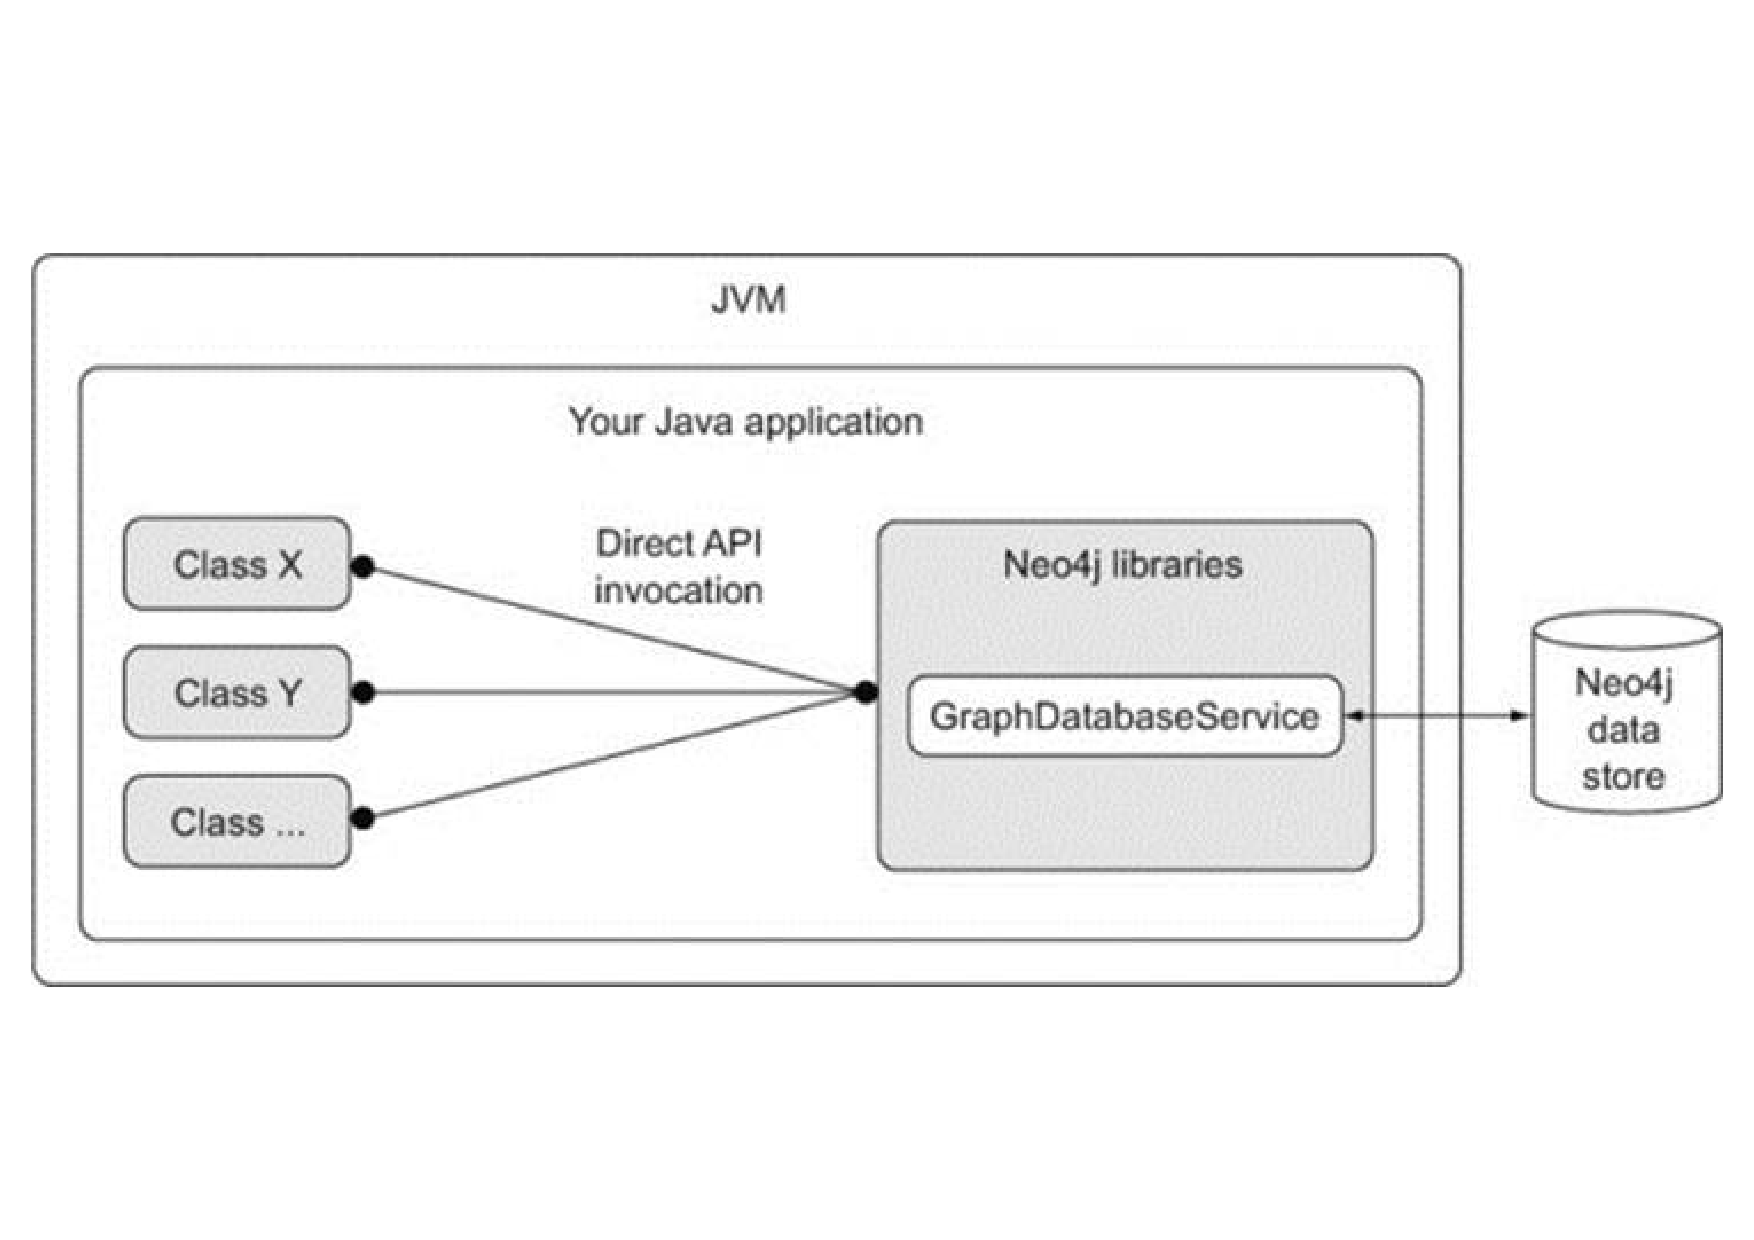
\includegraphics [width=12cm, height=10cm]{Figures/Embedded}
	\caption[Eingebettet]{Allgemeiner eingebetteteter Modus von Neo4j.}
	\label{fig:Embedded}
	\FloatBarrier
\end{figure}

\subsection{Der Server Modus}
Im Server Modus werden alle Anfragen von den Nutzern in einem eigenen Prozess verwaltet und mittels HTTP(Hypertext Transfer Protocol) als JSON-Formatiertes Dokument an die sogenannte REST API übermittelt \parencite{robinson2013graph}. Die REST API läuft in der Neo4j JVM und  verwaltet alle eintreffenden Anfragen der Nutzer und gibt diese an den GraphDatabaseService weiter, welcher die Bibliotheken verwaltet.
Dieser Modus ist für die Verwendung der High-Availability Fuktionen, welche das Nutzen der Datenbank auf mehren Systemen erlaubt, empfohlen\parencite{raj2015neo4j}. Da die Anfragen des Nutzer getrennt von der JVM der Neo4j Bibliotheken verwaltet werden und so mehrere Nutzer die Möglichkeit besitzen diese Funktionen zu Nutzen. Durch die  Übertragungsverzögerung innerhalb der Netzwerks und dem Übertragen durch eine weitere API ist der Geschwindigkeit langsamer als die des eingebetteten Modus. Dies wird in \ref{fig:Server} verdeutlicht.
\begin{figure}[!htb]
	\centering
	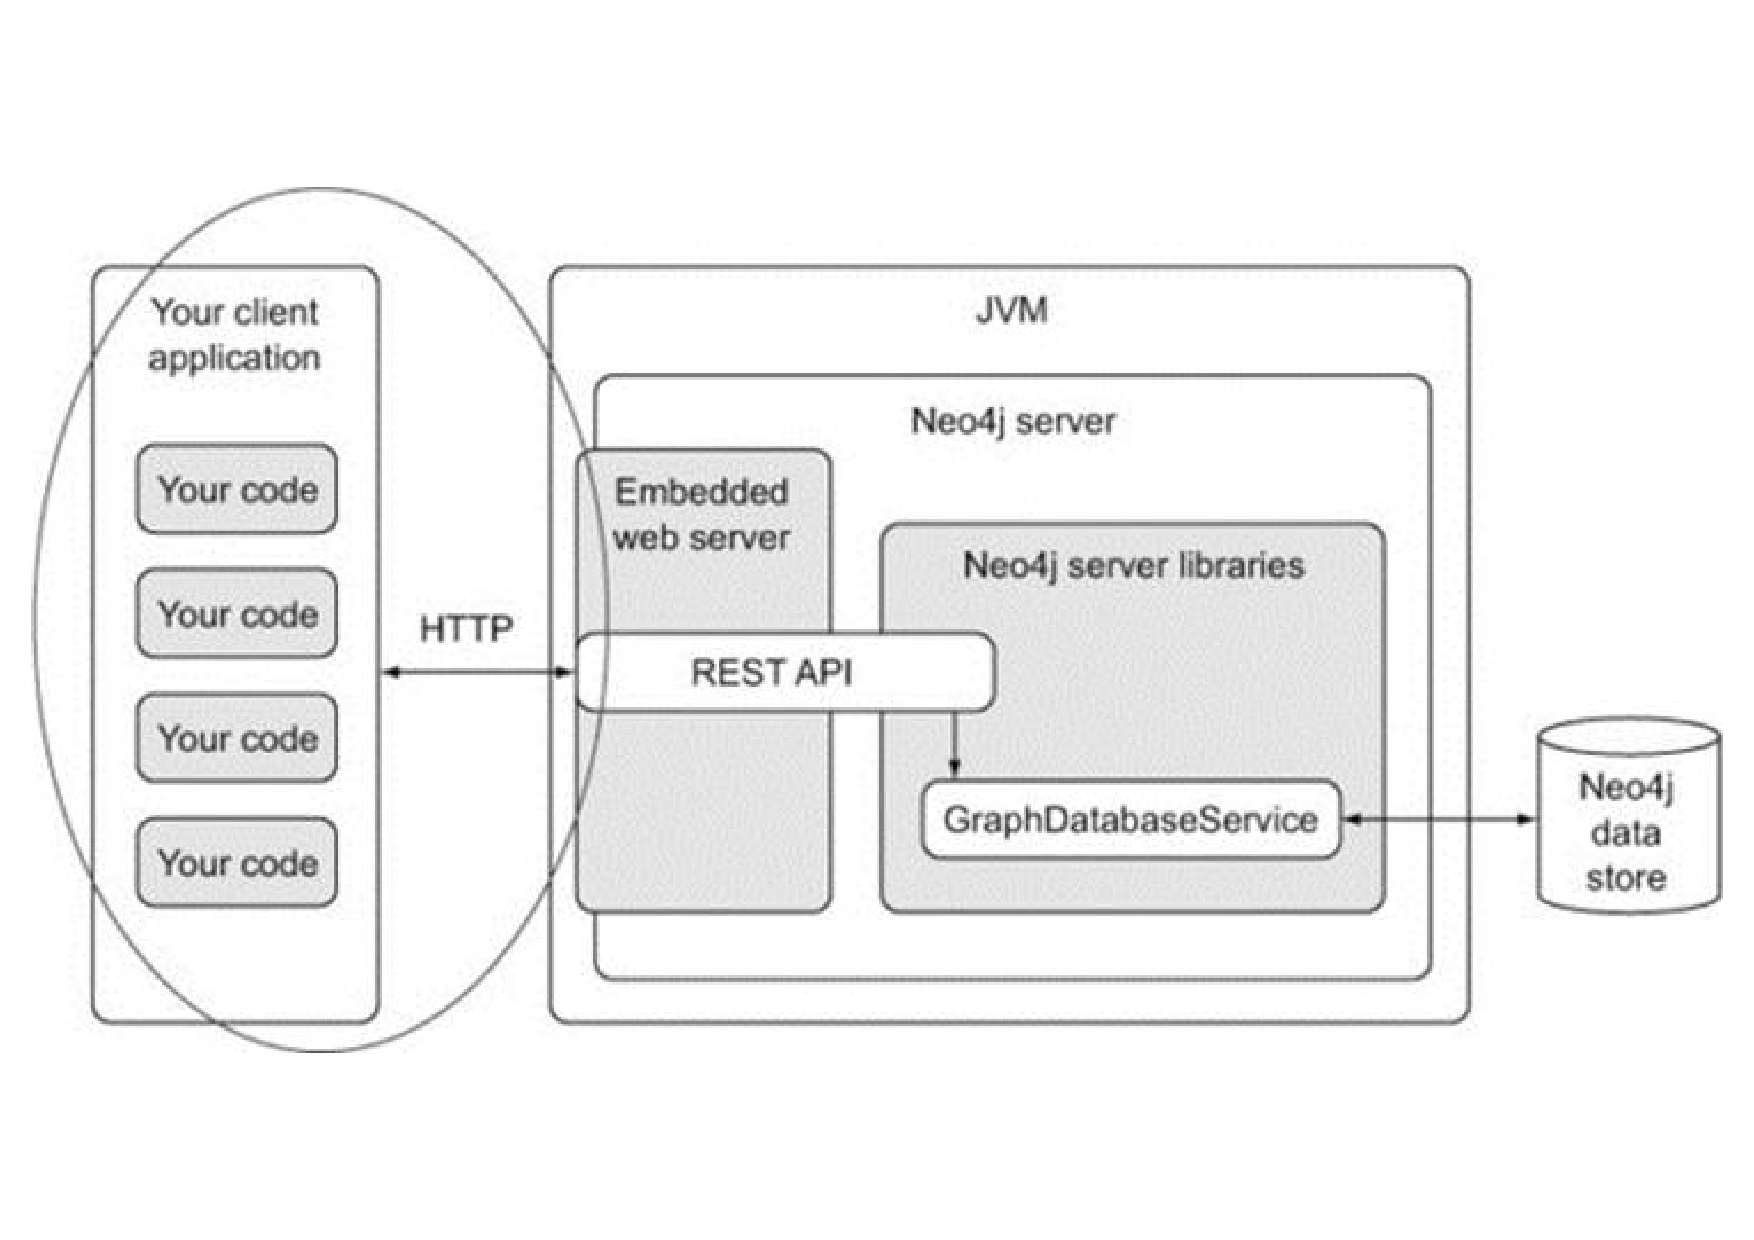
\includegraphics [width=14cm, height=12cm]{Figures/Server}
	\caption[Server]{Allgemeiner Servermodus von Neo4j.}
	\label{fig:Server}
	\FloatBarrier
\end{figure}


% Chapter Template

\chapter{Theoretische Grundlagen} % Main chapter title

\label{Kaptiel3} % Change X to a consecutive number; for referencing this chapter elsewhere, use \ref{ChapterX}

%----------------------------------------------------------------------------------------
%	SECTION 1
%----------------------------------------------------------------------------------------
\section{Vorraussetzungen}
Im Folgenden wird der verwendete Datensatz beschrieben und eine Kategorisierung der Anfragen für die folgenden Iterationen wird erläutert. 
\subsection{Datensatz}
Für die Evaluation wurde ein selbsterstellter Datensatz gewählt, dieser wurde aus folgendem Code erstellt \footnote{https://github.com/McHektor123/BA/blob/master/Neo4j/InitNeo4j2.java} unter Verwendung der Parameter \footnote{https://github.com/McHektor123/BA/blob/master/Constants/CONSTANTS.java}. Die Datenbank läuft im eingebettten Modus von Neo4j und besteht aus insgesamt 50.004 Entitäten, davon sind 4  vom Typ Action und  50000  vom Typ Person. Der Typen Action und Person besitzen 3 Eigenschaften, die erste ist 'name', welche aus einem String besteht, die zweite 'attribute besteht aus einem Int und die dritte 'time' ist vom Datentyp Date. Es gibt keine Entitäten, die eine Eigenschaft mit gleichen Wert besitzen. \newline
Es existieren insgesamt 4 Arten von Relationen: RELATIONSHIP1 und RELATIONSHIP2 bilden eine Relation von einer Entität des Typen Person zu einer Entität des Typen Action  und  RELATIONSHIP3 und RELATIONSHIP4 eine Relation von Person zu Person. Jede Person besitzt jeweils 1 Relation vom Typen RELATIONSHIP1 und eine vom Typen RELATIONSHIP2, wobei die Ziel-Actions disjunkt sind. Pro Person wurden 2.500 Relationen vom Typen RELATIONSHIP3 und 2.500 Relationen vom Typen RELATIONSHIP4 generiert, die Ziel-Personen sind nicht disjunkt. Jede Person besitzt 5002 Relationen. Da die Relationen als Kanten und die Entitäten als Knoten aufgefasst werden, besitzt der generierte Graph 50.004 Knoten und 250.100.000 Kanten mit einer physischen Gesamtgröße von 8.8 GB. 
\subsection{Anfragen}
Für die Evaluation werden die Anfragen nach  \parencite{angles2012comparison}  in folgende Kategorien unterteilt: Nachbarschafts-Anfragen, Erreichbarkeits-Anfragen, Muster-Passungs-Anfragen und  Zusammenfassungen. 
\begin{enumerate}
	\item Nachbarschafts-Anfragen: Es wird geprüft, ob ein Knoten direkt über eine  Kante mit einem anderen Knoten verbunden ist oder  es werden alle Knoten die über eine bestimmte Menge an Kanten erreichbar sind zu einer Menge zusammengefasst, dies ist auch als k-nächste Nachbarn Problem bekannt. Beide Fälle lassen sich auch auf die Verbundenheit von Kanten über Knoten übertragen.
	\item Erreichbarkeits-Anfragen: Die Suche nach einem Pfad, welcher 2 Knoten bzw. Kanten verbindet. Wenn ein Pfad besteht ist der Ziel-Knoten von dem Start-Knoten aus erreichbar, bei einem ungerichteten Graphen gilt auch der umgekehrte Fall. Beim dem Auffinden von mehreren Pfaden, entsteht zudem das Problem des Finden des kürzesten Pfades. Bei einem gewichteten Graphen kann dieses Problem um die Suche des schnellsten/leichtesten Pfades  erweitert werden. 
	\item Muster-Passungs-Anfragen: Prüfen, ob der Graph ein Sub-Graph enthält, welcher Ähnlichkeiten zu einem gegebenen Muster oder zu anderen Sub-Graphen aufweist. Dies ist als Graph bzw. Sub-Graph Isomorphismus bekannt. 
	\item Zusammenfassungen: Diese Anfragen fassen eine Ergebnismenge zu einem Wert zusammen, dies ist durch Funktionen wie MAX,AVG oder COUNT ,aber auch dem Lesen von Eigenschaften des Graphen wie die Menge alle Knoten, realisiert. 
\end{enumerate}
Eine Anfrage kann dabei mehrere Kategorien beinhalten. In der folgenden Evaluation werden die primär Grundanfragen der Kategorien 1,2 und 4 verwendet. Die gesamte Evaluation besteht aus 3 Iterationen, in denen eine Menge von Anfragen gestellt und analysiert werden. 
\section{Erste Iteration}
Die erste Iteration besteht primär aus Nachbarschafts-Anfragen und Zusammenfassungen. Im folgenden Abschnitt werden die Grundanfragen vorgestellt und es wird beschrieben wie daraus mehrere Anfragen gebildet werden. 
\subsection{Grundanfragen zur ersten Iteration}
\textbf{Grundanfrage 1.1} wird beschrieben als:
\begin{Verbatim}[frame=single]
 MATCH (X:Person)-[:RELATIONSHIP3]-(Y) 
 WHERE X.attribute>=250 AND Y.attribute>=15  
 RETURN COUNT(DISTINCT(Y))
\end{Verbatim} 
Grundanfrage 1.1 findet alle Personen, die über RELATIONSHIP3 erreichbar sind, unter der Voraussetzung dass bestimmte Bedingungen für die Eigenschaften 'attribute' erfüllt sind. Es handelt sich um eine Erreichbarkeits-Anfrage. Bei dieser Anfrage wird die Richtung der Relation RELATIONSHIP3 zu ausgehend,eingehend  geändert und zusätzlichen werden diese Anfragen  semantisch äquivalent in der JAVA Core API unter Verwendung der Traversal API formuliert. Bei den 3 in Cypher formulierten Anfragen wird die Relation RELATIONSHIP3 durch die Relation RELATIONSHIP2 ersetzt. Insgesamt entstehen 9 Anfragen aus Grundanfrage 1.1. \newline 
\textbf{Grundanfrage 1.2} wird beschrieben als: 
\begin{Verbatim}[frame=single]
MATCH (p:Person {name:'Person613'}) return p
\end{Verbatim} 
Diese Anfrage findet den Nutzer mit dem Namen "Person613". Sie wird dahingehend verändert, dass die Überprüfung des attributes 'name' in ein WHERE Prädikat verschoben wird und die Anfrage  in der Core API formuliert wird. Aus Grundanfrage 1.2 entstehen insgesamt 3 Anfragen.\newline 
\textbf{Grundanfrage 1.3} wird beschrieben als: 
\begin{Verbatim}[frame=single]
MATCH (X:Person{name: 'Person1'})-[:Relationship3]->(n1) 
WITH COLLECT(n1) as n 
MATCH (Y:Person{name: 'Person2'})-[:Relationship3]->(n1) 
WHERE n1 in n
RETURN COUNT(DISTINCT(n1))
\end{Verbatim} 
Diese Anfrage ermittelt alle gemeinsamen Nachbarn von Person1 und Person2, so ist es eine Nachbarschafts-Anfrage mit einer genutzten Zusammenfassung. Es entstehen insgesamt 3 Anfragen. Als Permutationen wird eine semantisch äquivalente Anfrage in den APIs und folgende in Cypher formuliert:
\begin{Verbatim}[frame=single]
 MATCH (X:Person{name: 'Person1'})-[:Relationship3]->(n1)
 		<-[:Relationship3]-(Y:Person{name: 'Person2'}) 
 RETURN COUNT(DISTINCT(n1))
\end{Verbatim} 
Für alle Anfragen, die mit der Traversal API geschrieben wurden, wird die Breadth-First-Methode für die Traversierungen verwendet. 
\subsection{Erwartungen zur ersten Iteration}
Im Folgenden werden Hypothesen über das Verhalten der Grundanfragen zur ersten Iteration aufgestellt und es werden  Begründungen ausgestellt. In dem praktischen Teil werden diese Hypothesen überprüft. \newline \newline
Für \textbf{Grundanfrage 1.1} entstehen 3 Aspekte, welche betrachtet werden.
\begin{enumerate}
\item Das Verhalten beim Ändern der Richtung der Relationen
\item Die Performanzunterschiede zwischen der Cypher und den APIs
\item Die Unterschiede zwischen der Anfrage mit Verwendung von RELATIONSHIP3 und RELATIONSHIP2.
\end{enumerate}
Zum 1. Aspekt: Es besteht die Vermutung, dass die Ausführungszeit am höchsten ist, wenn die Relation in beide Richtung gelten kann und die Zeit ist minimal wenn die Relation als ausgehende Kante beschrieben wird. \newline
 Zum 2. Aspekt: Wie in \parencite{raj2015neo4j} beschrieben, wird es empfohlen die APIs für eine erhöhte Performanz zu nutzen, da diese APIs nahe am Kern arbeiten und Cypher als Kern ferne Sprache in Neo4j aufgefasst wird. Aus diesem Grund wird erwartet, dass die Performanz bei den verwendeten Anfragen deutlich höher ist, wenn die Java Core API mit Verwendung der Traversal API genutzt wird. \newline
Zum 3. Aspekt: Da jede Person 1 Relation vom Typ RELATIONSHIP2 besitzt und maximal 2.500 vom Typ RELATIONSHIP3 wird Vermutet, dass die Anfragen mit der Relation RELATIONSHIP2 mindestens um den Faktor 100 schneller ausgeführt werden. \newline \newline
Für \textbf{Grundanfrage 1.2} werden 2 Aspekte betrachtet .
\begin{enumerate}
	\item Die allgemeine Performanz und die entstehenden Unterschiede für das Suchen eines Knotens
	\item Das Verhalten, wenn die Abfrage, nach dem Namen in das WHERE-Prädikat verschoben wird.
\end{enumerate}
Zum 1. Aspekt: Wie bei der Grundanfrage 1.1 wird vermutet, dass der Java Core API eine höhere Performanz besitzt, insbesondere weil keine Traversal API verwendet wurde. Alle 3 Anfragen werden eine sehr schnelle Ausführungszeit besitzen, da besonders der Gebrauch von Indizes ein schnelles Finden durch Eigenschaften erlaubt. \newline
Zum 2. Aspekt: Da der Optimizer nach Angaben der Neo4j Inc. \footnote{https://neo4j.com/blog/introducing-new-cypher-query-optimizer/ (27.06.19)} , die meisten Labels in das WHERE Prädikat verschiebt, sollte nur ein minimaler bis nicht vorhandener Performanzunterschied zwischen den beiden Anfragen bestehen. \newline \newline
Für \textbf{Grundanfrage 1.3} besteht ein Aspekt, der untersucht wird. 
\begin{enumerate}
	\item Ein Unterschied in der Laufzeit bei  semantisches Äquivalenz  
\end{enumerate}
Zum 1. Aspekt: Es wird vermutet, dass es keine signifikante Differenz zwischen den Laufzeiten gibt, falls ein Unterschied bestehen sollte, wird diese auf die Performanz des IN-Operator zurückgeführt.

\section{Zweite Iteration}
Die zweite Iteration verwendet die Nachbarschafts-Anfragen in einer erhöhten Tiefe , wodurch eine höherer Rechenaufwand simuliert wird. Es wird das Verhalten zwischen  Depth-First-Search und  Breath-First-Search betrachtet und die Bidirektionale Traversierung wird genutzt. Es werden komplexere Anfragen gestellt und es wird die Skalierbarkeit des Systems analysiert. 
\subsection{Grundanfragen zur zweiten Iteration}
\textbf{Grundanfrage 2.1} wird beschrieben als: 
\begin{Verbatim}[frame=single]
MATCH (p:Person{name :'Person1'})-[:RELATIONSHIP3*2]->(p1:Person) 
RETURN COUNT(DISTINCT(p1))
\end{Verbatim} 
Diese Anfrage findet die Anzahl aller Verbindungen über die Relation RELATIONSHIP3 mit der exakten Tiefe 2. Es handelt sich um eine Nachbarschafts-Anfrage. Diese Grundanfrage wird erneut mit der Tiefe 3 ausgeführt und beide Anfragen werden in den APIs mit der Breath-First-Search und Depth-First-Search ausgeführt. Es ergeben sich 6 Anfragen. \newline \newline
\textbf{Grundanfrage 2.2} wird beschrieben als: 
\begin{Verbatim}[frame=single]
MATCH t=(p:Person{name :'Person1'})-[:RELATIONSHIP3]->(p1:Person)
-[:RELATIONSHIP3]->(p2)
WHERE NOT (p)-[:RELATIONSHIP3]->(p2) 
RETURN COUNT(DISTINCT(p2))
\end{Verbatim} 
Diese Anfrage findet alle Personen, welche über die RELATIONSHIP3 mit dem direkten Nachbarn  p1 verbunden sind, aber nicht mit Person p verbunden sind. Ein Praktisches Szenario für diese Anfrage, wäre das Finden von neuen Freunden, die die Startperson nicht kennt. Diese Anfrage ist eine Erreichbarkeits- und Muster-Passungs Anfrage. Als Permutation wird eine semantisch äquivalente Anfrage in den APIs formuliert und es wird folgende Anfrage in Cypher formuliert:
\begin{Verbatim}[frame=single]
MATCH t=(p:Person{name :'Person1'})-[:RELATIONSHIP3*2]->(p1:Person)
WHERE NOT (p)-[:RELATIONSHIP3]->(p1)
RETURN COUNT(DISTINCT(p1))
\end{Verbatim} 
\textbf{Grundanfrage 2.3} wird beschrieben als: 
\begin{Verbatim}[frame=single]
MATCH (p:Person{name :'Person1'}),(p1:Person{name :'Person42'}),
		path=shortestPath((p)-[:RELATIONSHIP4*..3]->(p1)) 
RETURN LENGTH(path)
\end{Verbatim} 
Diese Anfrage gibt die Länge des kürzesten Pfades zwischen Person1 und Person42 über die Relation RELATIONSHIP4 an, die maximale Länge des Pfades soll   3 sein. Diese Anfrage ist eine Erreichbarkeits-Anfrage und nutzt den shortestPath Algorithmus von Cypher. Diese Anfrage wird erneut mit der Core API ausgeführt und als folgende Alternative in Cypher dargestellt: 
\begin{Verbatim}[frame=single]
MATCH (p:Person{name :'Person1'}),(p1:Person{name :'Person42'}),
		path=(p)-[:RELATIONSHIP4*..3]->(p1) 
RETURN LENGTH(path)
ORDER BY length(path) ASC LIMIT 1
\end{Verbatim}
Die alternative Formulierung von \textbf{Grundanfrage 1.3} wird in dieser Iteration als \textbf{Grundanfrage 2.4}  beschrieben :
\begin{Verbatim}[frame=single]
MATCH (X:Person{name: 'Person1'})-[:Relationship3]->(n1)
<-[:Relationship3]-(Y:Person{name: 'Person2'})
RETURN COUNT(DISTINCT(n1))
\end{Verbatim}
Die Anfrage findet gemeinsame Nachbarn zwischen der Person1 und Person2, dies ist eine  Nachbarschafts-Anfrage. Diese Anfrage wird mit der Breath-First- und Depth-First-Search formuliert und   wird zusätzlich mit der Bidirektionalen Traversierung bearbeitet. Es ergeben sich 3 Anfragen, da die in Cypher formulierte Anfrage nicht betrachtet wird. 
\subsection{Erwartungen zur zweiten Iteration}
Es werden Hypothesen zu den komplexeren Grundanfrage aus der zweiten Iteration vorgestellt und Ursache für das erwartete Verhalten werden aufgestellt. Diese Hypothesen werden in dem Teil zur praktischen Arbeit überprüft und die Ausführbarkeit von sehr rechenaufwendigen Anfragen wird getestet.  \newline \newline
Für \textbf{Grundanfrage 2.1} werden folgende Aspekte betrachet: 
\begin{enumerate}
	\item Ein Unterschied zwischen der Traversierung in den Tiefen 2 und 3 
	\item Das Verhalten von Breath-First und Depth-First
	\item Der relative Anteil an erreichten Personen im gesamten Graphen
\end{enumerate}
Zum 1. Aspekt: Bei der Anfrage in Cypher wird davon ausgegangen, dass die Zeit für die Traversierung mit der Tiefe 3 in quadratischer Abhängigkeit zu der  mit Tiefe 2 steht. Für  Breath-First und Depth-First besteht die Annahme, dass ein linearer Unterschied entsteht  und eine der beide Algorithmen signifikant schneller ausgeführt wird. \newline
Zum 2. Aspekt: Da der Graph ausgehend von dem Knoten der Person1 mit der Tiefe 3 eine relativ hohe Breite im Vergleich zu der Tiefe besitzt, wird vermutet dass die Anfrage mit Depth-First signifikant schneller  ausgeführt wird. \newline
Zum 3. Aspekt: Durch die Tiefe 2 können  unter der Annahme, dass alle Personen über die RELATIONSHIP3 genau 2500 Ziel-Personen besitzen, maximal 6.250.000 Knoten erreicht werden. Da der Graph 50.000 Personen-Knoten besitzt, gibt es eine hohe Redundanz unter den Ziel-Personen. Durch die theoretisch hohe Anzahl von zu erreichenden Knoten bei der Tiefe 2 wird vermutet ,dass alle Personen bei der Traversierung zur Tiefe 2 erreicht werden. \newline \newline
Für \textbf{Grundanfrage 2.2} werden folgende Aspekte betrachet: 
\begin{enumerate}
	\item Ein Unterschied in der Laufzeit bei  semantisches Äquivalenz  
	\item Die allgemeine Performanz von dem Ausdruck "WHERE NOT".
\end{enumerate}
Zum 1. Aspekt: Es wird vermutet, dass die Anfrage mit [RELATIONSHIP3*2] eine schneller Ausführungszeit besitzt, da dieser Ausdruck auf den Compiler optimiert ist. \newline
Zum 2. Aspekt: Da eine Weitere Anfrage im WHERE-Prädikat gestellt wird und beide Ergebnismengen verglichen werden, wird vermutet dass die Ausführungszeit sehr hoch ist. Durch die Eigenschaften des Multithreading wird die Anfrage in der Core-API um ein vielfaches schneller beantwortet werden. \newline  \newline
Für \textbf{Grundanfrage 2.3} werden folgende Aspekte betrachtet: 
\begin{enumerate}
	\item Die Berechnungszeit für den kürzesten Weg und die Länge von diesem
	\item Die Ausführungszeit in Cypher ohne Verwenden des Algorithmus
\end{enumerate}
Zum 1. Aspekt: Durch die Vermutung, dass alle Personen über RELATIONSHIP3/ RELATIONSHIP4 mit der Tiefe 2 erreicht werden können, wird davon ausgegangen dass der Pfad die Länge 1 oder 2 besitzen  wird. Die Ergebnisse werden mit den Ausführungszeiten von Grundanfrage 2.2 zusammenhängen und es wird keine höhere Ausführungszeit erwartet. \newline
Zum 2. Aspekt: Ausgehend von der Annahme,dass der Algorithmus für den Compiler optimiert ist, wird der Anfrage mit dem Algorithmus eine signifikant schnellere Ausführungszeit aufweisen als die Anfrage ohne gegebenen Algorithmus. \newline \newline
Für \textbf{Grundanfrage 2.4} wird folgender Aspekt betrachtet:
\begin{enumerate}
	\item Die relativen Berechnungszeit der 3 Traversierung-Methoden zueinander
\end{enumerate}
Zum 1. Aspekt: Durch die Größe des Graphen wird erwartet, dass die Bidirektionale Traversierung die kürzeste Bearbeitungszeit besitzen wird, da theoretisch die Hälfte der Berechnungsschritte notwendig ist. Ausgehend von den Vermutungen zur Grundanfrage 2.1 wird vermutet, dass die Anfrage mit Breath-First-Search die längste Berechnungszeit besitzen wird. 
\section{Dritte Iteration}
In der dritten Iteration werden alle Grundanfragen außer Grundanfrage 2.4 auf dem Datenbank managment system OrientDB \footnote{https://orientdb.com/} ausgeführt. Es werden die Laufzeiten der performantesten Formulierungen der Grundanfragen auf Neo4j mit den Zeiten gleichwertiger Anfragen auf dem System OrientDB verglichen. In OrientDB werden in dieser Evaluation alle Anfragen in SQL formuliert und evaluiert.  
\section{OrientDB}
OrientDB ist eine noSQL,  Multi-Model Datenbank von dem Entwickler OrientDB Ltd. Die Multi-Model Eigenschaft beschreibt die Fähigkeit, Daten als Dokumenten-Datenbank,Graph, Schlüssel/Wert-Modell oder als Objekte zu modellieren \footnote{http://orientdb.com/docs/3.0.x/misc/Overview.html}. Die Daten werde mittels API für eine unterstützte Sprache oder mit den Anfragensprachen Gremlin oder SQL manipuliert. Als direktes Eingabe-Interface steht das OrientDB Studio für den Browser zur Verfügung. OrientDB ist in der Community- und der Enterprise-Version verfügbar. Die Enterprise-Version verfügt über zusätzliche Features, die das Überwachen der Anfragen ermöglicht bzw. erleichtert. Da die Enterprise-Version über keine Features verfügt, die Einfluss auf die  Performanz haben, wurde für dieses Evaluation die Community Version gewählt. Die verwendete Version ist V 3.0.19. 
\subsection{Unterschiede von OrientDB und Neo4j}
Der primäre Unterschied ist, dass Neo4j eine reine Graphdatenbank ist und OrientDB eine Multi-Model Datenbank. Dadurch ist es OrientDB möglich beispielsweise Dokumente in die Datenbank einzupflegen und die gesamte Datenbank als Graphen zu verwalten. Neo4j verwaltet alle Daten in einem reinem Graph. Dadurch besitzen beide Datenbanken verschiedene Mengen von akzeptierten Daten \parencite{fernandes2018graph}. 
\newline
Die Datenbanken verwenden unterschiedlichen Anfragesprachen. OrientDB verwendet die standardisierte Anfragesprache SQL  mit Muster-Passung oder Gremlin und Neo4j verwendet die eigenen Sprachen Cypher. Cypher ist im Vergleich zu Gremlin oder SQLcnicht Turing-Vollständig \footcite{https://www.quora.com/Should-I-learn-Cypher-or-Gremlin-for-operating-a-Neo4j-database (29.07.19)}. 
\newline
Das sogenannte Sharding ist unter Neo4j nicht möglich. Sharding ermöglich das zerlegen einer Datenbank in mehere kleine Bestandteile. Diese Bestandteile können mit den gleichen Operatoren modelliert werden, wie der gesamte Graph

 
% Chapter Template

\chapter{Ergebnisse} % Main chapter title

\label{Kaptiel4} % Change X to a consecutive number; for referencing this chapter elsewhere, use \ref{ChapterX}

%----------------------------------------------------------------------------------------
%	SECTION 1
%----------------------------------------------------------------------------------------
\section{Versuchsaufbau}
Für die Ausführung der Anfragen wurde die Dell Precision Workstation T5500 verwendet. Das System besitzt 16 Prozessorkerne vom Typ Intel Xeon  X5500 mit je 2,66 GHz und  8 MB Level3 Cache. Insgesamt stehen 72 GB DDR3 RAM mit 1333 MHz zur Verfügung und das System läuft auf Ubuntu 18.04. Alle Datensätze werden auf einer SEAGATE ST3250318AS Festplatte mit insgesamt 250 GB Kapazität, 8 MB Cache und 7200 Umdrehungen pro Minute gespeichert.\newline
 Jede Anfrage des ersten Testlaufes wurde 50 mal ausgeführt und die Anfragen des zweiten Testlaufes wurden 25 mal ausgeführt. In OrientDB wurden alle Anfragen 25 mal wiederholt. Als repräsentativer Wert für die Bearbeitungszeit einer Anfrage  wurde das Arithmetische Mittel aus allen Wiederholungen gewählt. Bei der Berechnung wurde die Zeit für die allererste Ausführung einer Anfrage nicht berücksichtigt, da durch das Caching eine unverhältnismäßig hohe Bearbeitungszeit beim ersten Ausführen beobachtet wurde. In OrientDB ist die erste Bearbeitungen der Anfrage im Durschnitt ca. 43\% langsamer, als die Wiederholungen  der Anfragen. In Neo4j ist die erste Bearbeitung mit Cypher ca. 40 \% langsamer und mit der Core API ca. 17\% langsamer.  
\section{Auswertung}
Im folgenden Abschnitt werden Bearbeitungszeiten der Testläufe in Millisekunden tabellarisch präsentiert.  Darauf aufbauend werden die Hypothesen aus Kapitel 3 überprüft.  
\subsection{Ergebnisse des ersten Testlaufes}
Die Ergebnisse für Grundanfrage 1.1.1
\begin{Verbatim}[frame=single]
MATCH (X:Person)-[:RELATIONSHIP3]->(Y:Person) 
WHERE X.attribute>=250 AND Y.attribute>=15  
RETURN COUNT(DISTINCT(Y))
\end{Verbatim} 
 werden  in Tabelle \ref{tab:Query1_1} gezeigt. Durch die Bedingungen im Where-Prädikat entstehen im Vergleich zu den darauffolgenden Anfragen relativ hohe Bearbeitungszeiten. Die benötigte Bearbeitungszeit ist in allen drei Szenarien am längsten, wenn die Relationen in beide Richtungen betrachtet werden. Dies ist auf die hohe Anzahl der vorhandenen Relationen zurückzuführen. Bei der Anfrage in Cypher und der Core API für die RELATIONSHIP3  ist die Bearbeitungszeit bei der Suche für beide Richtungen länger als die Suchen für ausgehende und eingehende Kanten addiert. Für die Anfragen mit RELATIONSHIP3 ist die Zeit am geringsten, wenn die ausgehenden Kanten betrachtet werden. \newline
Die Anfrage für RELATIONSHIP3 wird mit der Core API in  allen Fällen fast doppelt so schnell berechnet wie in Cypher. Dieses Verhalten wird bei den weiteren Grundanfragen ebenfalls erwartet, da die Core API sehr nah an den Kernfunktionen von Neo4j arbeitet. \newline
Die Anfragen werden in Cypher für RELATIONSHIP2 etwas mehr als 1000 mal schneller als für REALTIONSHIP3 bearbeitet. Dies deutet auf eine gute Skalierbarkeit des Systems hin, da die Berechnungen beinahe linear zu der Anzahl der zu betrachtenden Relationen ansteigen. 
\FloatBarrier  
\begin{table}[h]
\centering
\begin{tabular}{ |p{3cm}||p{3cm}|p{3cm}|p{3cm}|  }
	\hline
	Anfrage& RELATIONSHIP3 &Core API&RELATIONSHIP2\\
	\hline
	Ausgehend	& 212620  & 82057   & 160\\
	Eingehend   & 215383    &123963&  64\\
	Beides&496704 & 222150&  165\\
	\hline
\end{tabular}
\caption{Ergebnisse der Grundanfrage 1.1.1}
\label{tab:Query1_1}
\end{table}
\FloatBarrier
 \noindent Die beobachteten Zeiten für Grundanfrage 1.2
 \begin{Verbatim}[frame=single]
 MATCH (p:Person {name:'Person613'}) return p
 \end{Verbatim} 
  in Tabelle \ref{tab:Query1_2} sind im Vergleich zu den Zeiten der anderen Grundanfragen sehr gering. Durch die geringe Anzahl von 50004 Knoten,dem Verwenden von Indizes und der konstanten Zugriffszeit entstehen die geringen Zeiten. \newline Entgegen der Hypothese entsteht ein hoher zeitlicher Unterschied, wenn sich die Bedingung im Where-Prädikat statt im Match-Prädikat 	befindet. Die beobachtete Bearbeitungszeit bei der Anfrage mit der Bedingung in dem Where-Prädikat ist drei mal schneller, als bei der Anfrage mit der Bedingung im Match-Prädikat. Da der Cypher Query Optimizer alle Bedingungen des Match-Prädikates in ein Where-Prädikat verschiebt, wird hier gezeigt, dass dieser Optimierungsschritt selber eine  Berechnungszeit in Anspruch nimmt. Für ein optimalen Gebrauch von Neo4j sollten dementsprechend alle Bedingungen direkt in einem Where-Prädikat formuliert werden, dies wird auch von den Entwicklern empfohlen \parencite{Optimizer}. \newline
In diesem Fall wird die Traversal API nicht genutzt, sondern nur die Core API. Eine Kernfunktion namens $findNodes()$ übernimmt die Suche nach einem Knoten mit angegebenen Eigenschaften, ohne dass der Nutzer das Vorgehen spezifizieren muss.  
\FloatBarrier
\begin{table}[h]
	\centering
		\begin{tabular}{ |p{3cm}|p{3cm}|p{3cm}|p{3cm}|  }
			\hline
			Ohne Where& Mit Where& Core API  \\
			\hline
			1,69   &  0,54  & 0,29  \\
			\hline
		\end{tabular}
		\FloatBarrier
		\caption{Ergebnisse der Grundanfrage 1.2}
		\label{tab:Query1_2}
\end{table}
 \vskip 2.5cm
\noindent Für Grundanfrage 1.3
\begin{Verbatim}[frame=single]
MATCH (X:Person{name: 'Person1'})-[:Relationship3]->(n1) 
WITH COLLECT(n1) as n 
MATCH (Y:Person{name: 'Person2'})-[:Relationship3]->(n1) 
WHERE n1 in n
RETURN COUNT(DISTINCT(n1))
\end{Verbatim} 
 wurde beobachtet, dass die semantisch äquivalente Anfrage ca. 1,57 mal schneller bearbeitet wird. Dies ist auf die effiziente Implementierung des IN-Operators zurückzuführen. Wie bei Grundanfrage 1.1.1 ist die Bearbeitung in der Core API schneller als in Cypher.
Die genauen Ergebnisse befinden sich in Tabelle	\ref{tab:Query1_3}.
\FloatBarrier
\begin{table}[h]
	\centering
		\begin{tabular}{ |p{3cm}|p{3cm}|p{3cm}|p{3cm}|  }
			\hline
			Grundanfrage & Äquivalent&Core API\\
			\hline
			 13,36    & 8,66 &  3,2\\
			\hline
		\end{tabular}
		\caption{Ergebnisse der Grundanfrage 1.3}
		\label{tab:Query1_3}
\end{table}
\FloatBarrier

\noindent Die normierte Verteilung aller Bearbeitungszeiten der Grundanfragen des ersten Testlaufes und ihrer Umformulierungen werden in Abbildung \ref{ref:Compare1} dargestellt. 

\begin{center}
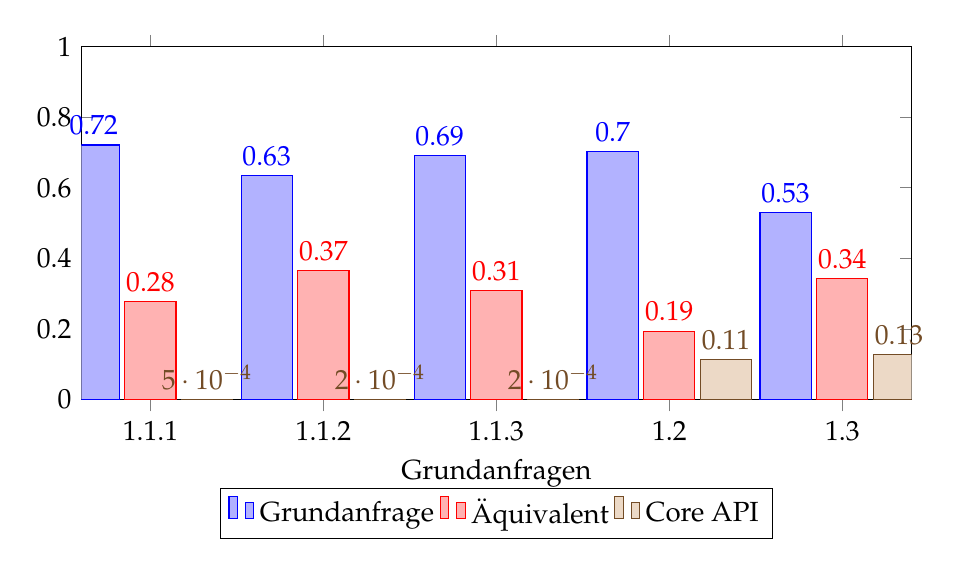
\begin{tikzpicture}
\centering
  \begin{axis}[
ybar,
bar width=.65cm,
width=\textwidth,
height=.5\textwidth,
legend style={at={(0.5,-0.25)},
	anchor=north,legend columns=-1},
symbolic x coords={1.1.1,1.1.2,1.1.3,1.2,1.3},
xtick=data,
nodes near coords,
nodes near coords align={vertical},
ymin=0,ymax=1,
xlabel={Grundanfragen},
]

\addplot coordinates {(1.1.2,0.6345) (1.1.1,0.7211)(1.1.3,0.6908)(1.2,0.7025) (1.3,0.5297)};
\addplot coordinates {(1.1.2,0.3652) (1.1.1,0.2783)(1.1.3,0.3089)(1.2,0.1935) (1.3,0.3434)};
\addplot coordinates{(1.1.2,0.0002)(1.1.1,0.0005)(1.1.3,0.0002)(1.2,0.1139)(1.3,0.1269)};
\legend{Grundanfrage,Äquivalent,Core API}
\end{axis}
\end{tikzpicture}
\captionof{figure}{Übersicht der Anfragen aus dem ersten Testlauf} 
\label{ref:Compare1}
\end{center}
\FloatBarrier

\subsection{Ergebnisse des zweiten Testlaufes}
In der Grundanfrage 2.1.1
\begin{Verbatim}[frame=single]
MATCH(p:Person{name:'Person1'})-[:RELATIONSHIP3*2]->(p1:Person) 
RETURN COUNT(DISTINCT(p1))
\end{Verbatim}
 werden bei der Traversierung in der Tiefe zwei ausgehend von Person1 99 \% aller Knoten des Graphen erreicht. Bei der Tiefe drei werden 100 \% der Knoten erreicht. Wie Tabelle \ref{tab:Query2_1} zeigt, wird mit Cypher die Traversierung in die Tiefe zwei ca. 64 mal schneller ausgeführt als die Traversierung in die Tiefe drei. In der Core API benötigt die Traversierung in die Tiefe drei mit der Breitensuche ca. 18 mal mehr Zeit als in die Tiefe zwei. Mit Verwendung der Tiefensuche benötigt die tiefere Traversierung nur 1,2 mal mehr Zeit. Da die Anzahl der zu betrachtenden Knoten um der Faktor 2500 ansteigt, besteht in allen Fällen kein linearer Zusammenhang zwischen der Bearbeitungszeit und der Anzahl der Knoten, die betrachtet werden müssen. \newline 
Es wird bestätigt, dass die Anfrage mit Tiefensuche  schneller als die Anfrage mit Breitensuche ausgeführt wird, in diesem Fall wird die Tiefensuche für Anfrage in der Tiefe zwei ca.18,4 mal schneller als Anfrage mit der Breitensuche ausgeführt. In der Tiefe drei wird die Tiefensuche ca. 277 mal schneller als die Breitensuche ausgeführt. Dies wird in Kapitel drei durch das Verhältnis der Breite zur Tiefe begründet. 
\FloatBarrier
\begin{table}[h]
\centering
		\begin{tabular}{ |p{3cm}||p{3cm}|p{3cm}|p{3cm}|  }
			\hline
			Anfrage& Cypher & Breitensuche&Tiefensuche\\
			\hline
			Tiefe 2   & 3501    & 1545&   84\\
			Tiefe 3&    223556  & 28318   & 102\\
			\hline
		\end{tabular}
		\caption{Ergebnisse der Grundanfragen 2.1.1 und 2.1.2}
		\label{tab:Query2_1}
\end{table}
\FloatBarrier
\noindent Wie Tabelle \ref{tab:Query2_2} zeigt, besteht ein geringer Unterschied zwischen Grundanfrage 2.2
\begin{Verbatim}[frame=single]
MATCH t=(p:Person{name :'Person1'})-[:RELATIONSHIP3]->(p1:Person)
-[:RELATIONSHIP3]->(p2)
WHERE NOT (p)-[:RELATIONSHIP3]->(p2) 
RETURN COUNT(DISTINCT(p2))
\end{Verbatim} 
 und der äquivalenten Anfrage in Cypher. Beide Anfragen sind um ein vielfaches langsamer als die Anfrage, die die Core API verwendet. In der Core API Anfrage werden zwei Ergebnismengen vom Java-typ Set gebildet und durch den Aufruf der Funktion removeAll() werden die Elemente der einen Mengen aus der anderen Menge entfernt. Dies entspricht einer Realisierung des Where not Ausdrucks in Java und wird schneller ausgeführt als der Ausdruck in Cypher. Alle drei Anfragen besitzen im Vergleich zu vorangegangen Anfragen eine extrem hohe Bearbeitungszeit.
\FloatBarrier
\begin{table}[h]
	\centering
		\begin{tabular}{ |p{3cm}|p{3cm}|p{3cm}|p{3cm}|  }
			\hline
			Grundanfrage 2.2 & Äquivalent&Core API\\
			\hline
			4740646    & 4753414 &  1609\\
			\hline
		\end{tabular}
		\caption{Ergebnisse der Grundanfrage 2.2}
		\label{tab:Query2_2}
\end{table}
\FloatBarrier
\noindent Der kürzeste Pfade, welcher in Grundanfrage 2.3
\begin{Verbatim}[frame=single]
MATCH (p:Person{name :'Person1'}),(p1:Person{name :'Person42'}),
path=shortestPath((p)-[:RELATIONSHIP4*..3]->(p1)) 
RETURN LENGTH(path)
\end{Verbatim} 
 untersucht wird, besitzt die Länge zwei. Die Grundanfrage 2.1.1 zeigt, dass bei einer Pfadlänge von zwei die meisten Knoten ausgehend von Person1 erreicht werden. Wie Tabelle \ref{tab:Query2_3} zeigt, ist die benötigte Bearbeitungszeit der Anfrage in Cypher unter Verwendung des gegebenen Algorithmus geringer als alle anderen Grundanfragen außer Grundanfrage 1.2. Erstmalig wird die Anfrage in Cypher schneller als die Formulierung in der Core API bearbeitet. Die Anfrage wird in Cypher 1,37 mal schneller beantwortet und  der absolute Unterschied zwischen den Bearbeitungszeiten beträgt 3,1 ms. Durch die geringe absolute Differenz ist es nicht garantiert, dass der kürzeste Pfad immer am schnellste mit Cypher berechnet wird. \newline
Die äquivalente Formulierung in Cypher besitzt die höchste aller beobachtetet Bearbeitungszeiten der gestellten Anfragen in Neo4j mit ca. 2,3 Stunden. Diese Formulierung ist eine naiver Ansatz ohne Verwendung des Algorithmus und besitzt viele Berechnungsschritten, die durch den Algorithmus entfallen. Zudem stoppt der Limit-Ausdruck nicht vorzeitig die Berechnung, sondern filtert die Ergebnismenge erst nach der Berechnung, dieses Verhalten ist mit der konservativen Stop-Strategie aus SQL zu vergleichen\parencite{carey1997saying}.   
\FloatBarrier
\begin{table}[!htb]
	\centering
		\begin{tabular}{ |p{3cm}|p{3cm}|p{3cm}|p{3cm}|  }
			\hline
			Grundanfrage 2.3 & Äquivalent&Core API\\
			\hline
			8,4    & 8370298 &  11,5\\
			\hline
		\end{tabular}
		\caption{Ergebnisse der Grundanfrage 2.3}
		\label{tab:Query2_3}
\end{table}
\FloatBarrier
\noindent Die Ergebnisse der Traversierungen des gesamten Graphen, wie in Grundanfrage 2.4.1
 \begin{Verbatim}[frame=single]
MATCH (a)-[RELATIONSHIP4]->(b) RETURN COUNT(DISTINCT(b))
\end{Verbatim}
 werden in Tabelle \ref{tab:Query2_4} dargestellt.
 In der Core API ist die bidirektionale Traversierung mit Breitensuche ca. 1,15 mal schneller als der gleiche Algorithmus bei einer einseitige Traversierung. Bei der Tiefensuche ist die bidirektionale Suche ca. 1,04 mal schneller. In beiden Fällen sind die einseitigen Traversierungen langsamer als die bidirektionale Alternativen. \newline
Trotz einer semantischen Äquivalenz von Grundanfrage 2.4.1 mit der Grundanfrage 2.1.2, bei der alle Knoten erreicht werden, ist eine höhere Bearbeitungszeit zu beobachten. 
\FloatBarrier
\begin{table}[!htb]
	\centering
	\begin{tabular}{ |p{5cm}||p{3cm}|p{3cm}|p{3cm}|  }
		\hline
		Anfrage & Zeit\\
		\hline
		Grundanfrage 2.4.1 & 284594\\
		\hline
		Vergleichsanfrage 1 & 31020  \\
		\hline
		Grundanfrage 2.4.2 & 31050\\
		\hline
		Grundanfrage 2.4.3 &   26982 \\
		\hline
		Grundanfrage 2.4.4 &  29558\\
		\hline
	\end{tabular}
	\caption{Ergebnisse der Grundanfragen 2.4.1-2.4.4}
	\label{tab:Query2_4}
\end{table}
\FloatBarrier

\subsection{Ergebnisse des dritten Testlaufes}
Für die folgenden Aussagen werden die Werte aus der Tabelle \ref{tab:Query3}  betrachtet. Diese Tabelle stellt die Bearbeitungszeiten der Grundanfragen, ihrer Äquivalente in der Core API und in der OrientDB dar. \newline
Die Grundanfragen 1.1.1-1.1.3 werden in Cypher durchschnittlich ca. 12 mal schneller ausgeführt als in der OrientDB, die relativ langen Bearbeitungszeiten bei beiden Systemen entstehen durch die Bedingungen im Where-Prädikat. In allen Fällen benötigt die Grundanfrage 1.1.3, welche die eingehenden und ausgehenden Kanten betrachtet, die längste Zeit zur Bearbeitung. Dies zeigt, dass OrientDB und Neo4j durch das Einfügen einer Bedingung im Where-Prädikat und der Anzahl der zu betrachtenden Kanten beeinflusst werden und bei solchen Anfragen aufwendige Berechnungen ausführen. \newline
 Grundanfrage 1.2, welche solange über den Graphen traversiert bis ein gegebener Knoten gefunden ist, weist in OrientDB eine schnellere Bearbeitungszeit als Neo4j mit der Core API oder Cypher auf und wird ca. 3,7 mal schneller bearbeitet als die in Cypher gestellte Anfrage. Dies lässt sich mit einer effizienteren Implementierung der Indizies erklären. Die Anfrage wird in allen Fällen in weniger als einer Millisekunde beantwortet und bildet die am schnellsten beantwortete Anfrage. \newline
Grundanfrage 1.3, welche eine einfache Anfrage zum Finden von gemeinsamen Nachbarn darstellt, besitzt in Cypher und der Core API eine relativ geringe Bearbeitungszeit in der Größenordnung von einigen Millisekunden. In OrientDB befindet sich Grundanfrage 1.3 mit einer benötigten Zeit von 83955 ms in einer anderen Größenordnung und deutet darauf hin, dass der Vergleich von zwei Mengen miteinander in Neo4j effizienter implementiert ist. Dies ist auch in Grundanfrage 2.2 zu beobachten, für diese Anfrage muss bis in die Tiefe zwei traversiert werden und zwei Mengen müssen miteinander verglichen werden. Die Anfrage besitzt eine extrem hohe Bearbeitungszeit von mehreren Stunden, obwohl das Traversieren in der Tiefe zwei, wie bei Grundanfrage 2.1.1 mit 72092 ms zu beobachten, eine relativ geringe Zeit benötigt, der Vergleich der beiden Mengen bildet so den rechenaufwendigeren Schritt. \newline
 Grundanfrage 2.1.1 wird in Cypher ca. 20,6 mal schneller bearbeitet als in der OrientDB. Grundanfrage 2.1.2 wird in der OrientDB ca. 2,1 mal schneller beantwortet. Dies deutet darauf hin, dass OrientDB besser skaliert als Neo4j mit Cypher. In OrientDB wird die Grundanfrage 1.1.2 ca. 1,5 mal langsamer ausgeführt als Grundanfrage 1.1.1, in Neoj4 wird diese Anfrage ca. 60,9 mal langsamer ausgeführt.   Die Grundanfrage 2.1.2 ist mit der Grundanfrage 1.2 die einzige Grundanfrage, die in OrientDB schneller bearbeitet wird, als in Neo4j mit Cypher. \newline  
 Grundanfrage 2.2 konnte in dieser Evaluation nicht vollständig analysiert werden, da die erste Ausführung der Anfrage ohne Caching ungefähr 70 Stunden benötigt hat. Weitere Wiederholungen mit Caching waren nicht möglich, aber würden bei der durchschnittlichen Verkürzung der Bearbeitungszeit durch das Caching von ca. 43\%  ungefähr 40 Stunden benötigen . \newline
OrientDB benötigt mit 37,6 ms für Grundanfrage 2.3  wie Neo4j eine relativ kurze Zeit von einigen Millisekunden zur Bearbeitung, dies lässt sich durch eine effiziente Implementierung des shortestpath-Algorithmus erklären. Das Finden des kürzesten Pfades ist ein grundlegendes Problem bei Graphen und der Algorithmus wurde bereits in der OrientDB Version 1.7.8 vom 13. August 2014 veröffentlicht \parencite{Old_OrientDB}. Durch die frühe Zurverfügungstellung ist es wahrscheinlich, dass der Algorithmus mit einer effizienten Implementierung veröffentlicht wurde oder über die Jahre optimiert wurde. \newline
Für die Grundanfrage 2.4.2, welche mit Breitensuche über den gesamte Graphen traversiert, ist nur ein Vergleich zwischen OrientDB und der Core API von Neo4j möglich, da der Such-Algorithmus in Cypher nicht explizit angegeben werden kann und immer Tiefensuche verwendet wird. Durch die gleiche Komplexität von O(V+E) bei der Tiefen- und Breitensuche, benötigen die Grundanfragen 2.4.1 und 2.4.2 in OrientDB eine gleich lange Bearbeitungszeit. In Cypher wird die Grundanfrage 2.4.1 ca. 2,7 mal schneller bearbeitet als die gleiche Anfrage in OrientDB. Mit Verwendung der Core API wird die einseitige Tiefen- und Breitensuche durchschnittlich ca. 24.8 mal schneller beantwortet als in OrientDB. \newline
 Unter der Berücksichtigung aller beobachteten Zeiten außer von Grundanfrage 2.2 werden die Anfragen mit der Core API durchschnittlich ca. 207 mal schneller bearbeitet als in OrientDB und mit Cypher ca. 1,9 mal schneller als OrientDB. 
\FloatBarrier
\begin{table}[h]
	\centering
	\begin{tabular}{ |p{6cm}||p{2cm}|p{2cm}|p{2cm}|  }
		\hline
		Anfrage& Cypher & OrientDB & Core API \\
		\hline
	Grundanfrage 1.1.1  & 215383 & 3495459    &  64\\
	Grundanfrage 1.1.2& 212620 & 1674758   & 160   \\
	Grundanfrage 1.1.3& 496704 & 6350806 & 165  \\
	Grundanfrage 1.2& 0,54 & 0,17   & 0,29   \\
	Grundanfrage 1.3 & 8,66& 83955  & 3,2    \\
	Grundanfrage 2.1.1& 3501 & 72092   & 84   \\
	Grundanfrage 2.1.2& 234132& 110064  & 102    \\
	Grundanfrage 2.2& 4740646 &  $\approx$ 40h   & 1609  \\
	Grundanfrage 2.3& 8,4  & 37,6   & 11,5   \\
	Grundanfrage 2.4.1& 284594 & 768830  & 31050\\
	Grundanfrage 2.4.2& -  & 774040   & 31020   \\
		\hline
	\end{tabular}
	\caption{Ergebnisse der Grundanfragen auf Neo4j und OrientDB}
	\label{tab:Query3}
\end{table}
\FloatBarrier
\section{Anwendungsszenario}
Neoj4 Inc. stellt zahlreiche Nutzungen von Graphen in verschiedenen Themenkomplexen vor \parencite{Examples}. Für jeden Themenkomplex werden mehrere Beispielgraphen von eigenständigen Entwicklern, welche nicht für Neo4j arbeiten, zur Verfügung gestellt. Das folgende Anwendungsszenario stellt den Zweck einer Graphdatenbank für Kinofilme dar.\newline
In diesem Beispiel ist der Nutzer ein Betreiber eines Kinos, welches aktuelle Kinofilme ausstrahlt und spezielle Veranstaltungen bietet. Bei diesen Veranstaltungen werden mehrere Filme von einer Kategorie oder einem bestimmten Schauspieler oder Regisseur gezeigt. Diese Veranstaltungen werden mehrere Wochen vor dem Veranstaltungstermin verplant und finden über mehrere Tage statt. Solche Veranstaltungen wurden schon mehrmals betrieben und die Planung besitzt einen routinierten Ablauf, sodass viele Schritte effizient bearbeitet werden. Der zeitaufwendigste Arbeitsschritt, stellt das Finden von Filmen für das Veranstaltungsprogramm dar. \newline
Aktuell stellt der Kinobetreiber eine Liste von Filmen für die Veranstaltung manuell zusammen, hierfür werden Filme ausgewählt, die der Betreiber selber kennt und es werden verschiedene Quellen aus dem Internet für eine Auswahl verwendet. Die Liste besitzt die Namen der Filme, zusätzliche Informationen wie die Länge eines Filmes sind durch die Vielzahl von Quellen nicht immer vorhanden. Fehlende Informationen müssen für eine optimale Planung des Kinoprogramms erneut herausgesucht werden und einige Filme müssen nach dem initialen Aufstellen der Liste  aussortiert werden. \newline  
Für eine Beschleunigung dieses Arbeitsschrittes kann Neo4j verwendet werden. Unabhängig von dem Betriebssystem steht die kostenfreie Anwendung $Neo4j\; Desktop$ zur Verfügung. Durch diese Anwendung für den Desktop ist die Bedienung von Neo4j über ein grafischen User Interface(GUI) möglich. Zusätzlich wird die Erweiterung $APOC$ benötigt, welche per Mausklick in $Neo4j\; Dekstop$ eingebunden werden kann. Mit dieser Erweiterung ist es möglich Daten mit verschiedenen Dateiformaten wie CSV oder JSON in die lokale Neo4j Datenbank zu importieren. Für das Thema Kino stehen im Internet zahlreiche, große Datensätze mit Filmen kostenfrei zur Verfügung \parencite{Kaggle}. Nach dem Importieren eines solchen Datensatzes, kann der Nutzer durch die Eingabemaske eine Anfrage stellen, um so eine übersichtliche vollständige Liste von Filme zu erhalten. Folgende Anfrage erstellt eine Liste von 20 Filmen mit dem Thema Verbrechen: 
\begin{Verbatim}[frame=single]
MATCH(m:Film) 
WHERE m.Genre = 'Verbrechen' or m.Plot contains 'Verbrechen'
RETURN m.Name as Name, m.Regie as Regie, 
	m.Länge as Länge, m.Plot as Plot 
LIMIT 20
\end{Verbatim}
Bei einem hohen Erfolg der Veranstaltung können ausgehend von den gezeigten Filmen Schauspieler aus diesen Filmen gefunden werden:
\begin{Verbatim}[frame=single]
MATCH (s:Schauspieler)-[SpielteIn]->(m:Film)
WHERE m.Genre = 'Verbrechen' or m.Plot contains 'Verbrechen'
RETURN s.Name as Name, count(m) as Anzahl_der_Filme,
Order by count(m) desc
LIMIT 10
\end{Verbatim}
Es werden 10 Schauspieler gefunden, die in den meisten Filmen zum Thema Verbrechen mitgespielt haben. Diese Schauspieler sind potenzielle Kandidaten für eine Veranstaltung, bei der nur Filme von diesen Schauspielern gezeigt werden. Durch Bedingungen bezüglich eines Attributes wie der Bewertung eines Filmen, kann die Auswahl weiter eingegrenzt werden.
\begin{Verbatim}[frame=single]
MATCH (s:Schauspieler)-[SpielteIn]->(f:Film) 
WHERE s.name = 'Christian Bale' AND f.Bewertung >= 5
RETURN f.Name as Name, f.Regie as Regie, 
	f.Länge as Länge, f.Plot as Plot 
LIMIT 20
\end{Verbatim}
Neo4j übernimmt die Auswertung eines Datensatzes, der in einem CSV Format dargestellt wird und von dem Nutzer nicht schnell verwendet werden kann. Durch die effiziente Implementierung von Neo4j wird in kurzer Zeit eine vollständige Liste mit Filmen erstellt. Der Arbeitsschritt zum Erstellen einer Liste mit geeigneten Filmen wird damit beschleunigt und effizienter ausgeführt.
\section{Limitierungen und zukünftige Arbeit}
Die durchgeführte Evaluation nutzt mit OrientDB  eine einzige Referenzdatenbank. Dies ist keine reine GDB und unterstützt eine erweiterte Verwaltung der Daten. Für eine näherer Einordnung der Performanz von Neoj4 ist ein Vergleich mit einer reinen GDB wie beispielsweise der Sparksee Database sinnvoll \parencite{Sparksee}. Diese Datenbank konnte in dieser Evaluation auf Grund von Kommunikationsprobleme mit Sparsity technologies nicht verwendet werden. Durch einen Vergleich mit der Sparksee Database könnte die Performanz von zahlreichen Graphalgorithmen  wie Zentralitäts-Algorithmen, zur Erkennung von Gruppen mit gemeinsamen Eigenschaften, überprüft werden. Dies ist mit OrientDB nicht möglich, da keine vergleichbare Implementierung der von Neo4j unterstützen Graphalgorithmen im vollen Ausmaß in OrientDB gegeben ist. \newline 
Ein Vergleich zwischen Neo4j und einer relationalen Datenbank, wie in \parencite{vicknair2010comparison} beschrieben, ist für eine weitere Beschreibung der Vor- und Nachteile einer GDB sinnvoll. Dieser Vergleich wurde aus zeitlichen Gründen nicht vollzogen. Die Referenz zur OrientDB hat einen Vergleich zu einer anderen noSQL-Datenbank dargestellt und so ein erste Einschätzung zu der Performanz von Neo4j ermöglicht. \newline
Ein weitere zu betrachtender Aspekt, ist das Ausführen einer Neo4j Datenbank im Server Modus auf mehreren Geräten verteilt. Durch diesen Aspekt können die ACID und CAP Eigenschaften untersucht werden und die Grenzen einer verteilten Neo4j-Datenbank getestet werden. Zudem kann ein Vergleich zwischen der Datenbank im eingebetteten Modus und dem Server Modus durchgeführt werden. So können Vor- und Nachteile und  Anwendungsszenarien spezifiziert werden. \newline
Eine kleinerer nicht betrachteter Aspekt ist die temporale Eigenschaft von Neo4j. Der vorgestellte Datensatz besitzt ein Attribut vom Typen Date und stellt so eine temporale Datenbank dar, es fehlt ein Testlauf mit Anfragen zu diesem Attribute. Eine Allgemeine Betrachtung des temporalen Verhalten der Datenbank ist für eine genauere Einordnung von Neo4j im Vergleich zu anderen temporalen Graphdatenbanken sinnvoll.   \newline
Die Anfragesprache GraphQL wird als standardisierte Anfragesprache für GDBs angesehen \parencite{GraphQL}. In der Zukunft sollte GraphQL auch in Neo4j getestet werden, dies ist mit einer Erweiterung für Neo4j möglich und erfordert die Verwendung einer weiteren API. In dieser Evaluation wurde GraphQL nicht verwendet. 
\section{Fazit}
Neo4j unterstützt mit den Java-Standardtypen und zahlreichen zeitlichen Typen wie Time, LocalTime oder DateTime eine Vielzahl von Datentypen, welche für die Modellierungen von Daten notwendig sind \parencite{Types}. Durch die Zurverfügungstellung der Anwendungen Neo4j Dekstop und Neo4j Browser und einer dazu gegebenen Anfragesprache, werden die benötigten Kenntnisse zur Bedienung des System minimiert. Für eine spezifischeren Gebrauch der Datenbank, werden mehrere Programmiersprachen unterstützt. Durch diese Schnittstellen ist es mögliche, das System auf viele Weisen zu nutzen und eine große Zielgruppe kann das System für viele Zwecke verwenden. \newline 
Der erste und zeite Testlauf zeigen, dass dem Gebrauch der APIs in fast allen Fällen zu einer besseren Performanz führt. Mit Verwendung der Traversal API besitzt der Nutzer eine flexible Möglichkeit die Performanz seiner Anfragen zu beeinflussen. So ist es möglich zwischen Breiten- und Tiefensuche zu wählen. Die am schnellsten bearbeiteten Anfragen besitzen keine gemeinsame Kategorie von den vorgestellten Kategorien aus Absatz \ref{Kategorien}. Die am langsamsten bearbeiteten Anfragen besitzen ebenfalls keine gemeinsamen Kategorien. Grundanfrage 2.2, welche die einzige Mustervergleichs-Anfrage ist, besitzt eine besonders hohe Bearbeitungszeit. Dementsprechend lässt sich nur für Mustervergleichs-Anfragen ein Bezug von Anfragen-Kategorie und Bearbeitungszeit in Neo4j erkennen, die anderen Kategorien weisen keinen solchen Bezug auf. \newline
Wie die Tabellen \ref{tab:Query1_2} und \ref{tab:Query2_3} zeigen, können semantisch gleiche Anfragen in Cypher Unterschiede in ihrer Performanz aufzeigen. Dieses Verhalten ist in den APIs ebenfalls zu beobachten. Das System lässt sich durch eine hohe Anzahl von Schnittstellen leicht benutzen, aber das System effektiv zu nutzen und eine Anfrage effizient ausführen zu lassen, ist nicht trivial und erfordert technologische Kenntnisse. Durch Hinweise von Neo4j Inc. werden einige Möglichkeiten für das effiziente Ausführen gegeben \parencite{Optimizer}. Diese Hinweise befassen sich teilweise mit dem Umformulieren der Anfragen, um die benötigten Arbeitsschritte des Optimierers zu minimieren. Wie in den Ergebnissen zur Grundanfrage 1.2 erläutert, deutet dies auf einen inperformanten Optimierer hin. \newline
Im Vergleich zu der Muli-model Datenbank OrientDB unter Verwendung von SQL besitzt Neo4j mit der Core API und Cypher ein bessere Performanz. Der verwendete Datensatz ist unter Neo4j ca. 2.4 mal größer als bei OrientDB. Allgemein besitzt Neo4j so eine bessere Performanz, aber die Speicherverwaltung unter Neo4j ist schlechter. Eine Einschätzungen über die Performanz im globalen Kontext verglichen mit mehreren anderen Datenbankmanagementsystemen ist, wie in \parencite{jouili2013empirical} ausgeführt, kann Rahmen dieses Evaluation nicht getroffen werden. 

\begin{acknowledgements}
	An dieser Stelle möchte ich all jenen danken, die durch ihre fachliche und persönliche Unterstützung zum Gelingen dieser Bachelorarbeit beigetragen haben. \newline \newline
	Ebenso gilt mein Dank meinen Freunden und Bekannten für das Korrekturlesen. Zuletzt möchte ich noch all denjenigen danken, die in der Zeit der Erstellung dieser Arbeit für mich da waren, insbesondere meinen Freunden. \newline \newline
	Schließlich danke ich meinen Freunden während der Studienzeit für drei sehr schöne Jahre in Lübeck.
\end{acknowledgements}
%\include{Chapters/Chapter4} 
%\include{Chapters/Chapter5} 

%----------------------------------------------------------------------------------------
%	THESIS CONTENT - APPENDICES
%----------------------------------------------------------------------------------------

\appendix % Cue to tell LaTeX that the following "chapters" are Appendices

% Include the appendices of the thesis as separate files from the Appendices folder
% Uncomment the lines as you write the Appendices

%% Appendix A

\chapter{Frequently Asked Questions} % Main appendix title

\label{AppendixA} % For referencing this appendix elsewhere, use \ref{AppendixA}

\section{How do I change the colors of links?}

The color of links can be changed to your liking using:

{\small\verb!\hypersetup{urlcolor=red}!}, or

{\small\verb!\hypersetup{citecolor=green}!}, or

{\small\verb!\hypersetup{allcolor=blue}!}.

\noindent If you want to completely hide the links, you can use:

{\small\verb!\hypersetup{allcolors=.}!}, or even better: 

{\small\verb!\hypersetup{hidelinks}!}.

\noindent If you want to have obvious links in the PDF but not the printed text, use:

{\small\verb!\hypersetup{colorlinks=false}!}.

%\include{Appendices/AppendixB}
%\include{Appendices/AppendixC}

%----------------------------------------------------------------------------------------
%	BIBLIOGRAPHY
%----------------------------------------------------------------------------------------

\printbibliography[heading=bibintoc]

%----------------------------------------------------------------------------------------

\end{document}  
